\documentclass[]{elsarticle} %review=doublespace preprint=single 5p=2 column
%%% Begin My package additions %%%%%%%%%%%%%%%%%%%
\usepackage[hyphens]{url}

  \journal{Transportation Research Part D: Transport and Environment} % Sets Journal name


\usepackage{lineno} % add
\providecommand{\tightlist}{%
  \setlength{\itemsep}{0pt}\setlength{\parskip}{0pt}}

\usepackage{graphicx}
\usepackage{booktabs} % book-quality tables
%%%%%%%%%%%%%%%% end my additions to header

\usepackage[T1]{fontenc}
\usepackage{lmodern}
\usepackage{amssymb,amsmath}
\usepackage{ifxetex,ifluatex}
\usepackage{fixltx2e} % provides \textsubscript
% use upquote if available, for straight quotes in verbatim environments
\IfFileExists{upquote.sty}{\usepackage{upquote}}{}
\ifnum 0\ifxetex 1\fi\ifluatex 1\fi=0 % if pdftex
  \usepackage[utf8]{inputenc}
\else % if luatex or xelatex
  \usepackage{fontspec}
  \ifxetex
    \usepackage{xltxtra,xunicode}
  \fi
  \defaultfontfeatures{Mapping=tex-text,Scale=MatchLowercase}
  \newcommand{\euro}{€}
\fi
% use microtype if available
\IfFileExists{microtype.sty}{\usepackage{microtype}}{}
\bibliographystyle{elsarticle-harv}
\ifxetex
  \usepackage[setpagesize=false, % page size defined by xetex
              unicode=false, % unicode breaks when used with xetex
              xetex]{hyperref}
\else
  \usepackage[unicode=true]{hyperref}
\fi
\hypersetup{breaklinks=true,
            bookmarks=true,
            pdfauthor={},
            pdftitle={Examining horizontal and vertical equity to a public bicycle share program using a balanced floating catchment area accessibility approach},
            colorlinks=false,
            urlcolor=blue,
            linkcolor=magenta,
            pdfborder={0 0 0}}
\urlstyle{same}  % don't use monospace font for urls

\setcounter{secnumdepth}{0}
% Pandoc toggle for numbering sections (defaults to be off)
\setcounter{secnumdepth}{0}

% Pandoc citation processing

% Pandoc header
\usepackage{booktabs}
\usepackage{longtable}
\usepackage{array}
\usepackage{multirow}
\usepackage{wrapfig}
\usepackage{float}
\usepackage{colortbl}
\usepackage{pdflscape}
\usepackage{tabu}
\usepackage{threeparttable}
\usepackage{threeparttablex}
\usepackage[normalem]{ulem}
\usepackage{makecell}
\usepackage{xcolor}



\begin{document}
\begin{frontmatter}

  \title{Examining horizontal and vertical equity to a public bicycle share
program using a balanced floating catchment area accessibility approach}
    \author[McMaster University]{Elise Desjardins\corref{1}}
   \ead{desjae@mcmaster.ca} 
    \author[University of Toronto Scarborough]{Christopher D. Higgins}
   \ead{cd.higgins@utoronto.ca} 
    \author[McMaster University]{Antonio Paez}
   \ead{paezha@mcmaster.ca} 
      \address[McMaster University]{School of Earth, Environment \& Society, McMaster University, 1280 Main
Street West, Hamilton, ON L8S4L8}
    \address[University of Toronto Scarborough]{Department of Geography \& Planning, University of Toronto Scarborough,
1265 Military Trail, Toronto, ON M1C1A4}
      \cortext[1]{Corresponding Author}
  
  \begin{abstract}
  Public bicycle share programs (PBSPs) can play a role in advancing
  transportation equity if they make cycling more accessible to
  disadvantaged populations. In Ontario, the City of Hamilton expanded
  their PBSP in 2018 by adding twelve docking stations with the explicit
  objective of increasing spatial equity in access. In this case study, we
  investigate differentials in accessibility to stations using a balanced
  floating catchment area accessibility approach and compare accessibility
  with and without the equity stations. We analyze micro zones to better
  reflect walking to a station and conduct a sensitivity analysis at
  several walking time thresholds. We then reaggregate the estimated
  accessibility for further analysis using census data. Our findings
  indicate that equity stations increased the serviced population at every
  threshold examined. Although accessibility increased for the whole
  population, this increase was relatively modest especially for
  population in the bottom 20\% of median total household income.
  \end{abstract}
  
 \end{frontmatter}

\newpage

\hypertarget{introduction}{%
\section{1. Introduction}\label{introduction}}

The potential of public bicycle share programs (PBSPs) to increase
cycling levels is but one of many reasons for implementing such programs
in urban areas (Hosford et al., 2018, 2019). As a healthy, inexpensive,
and convenient form of public transportation, shared bicycles can
encourage individuals to take up cycling for short local trips or first
and last mile trips to other public transportation instead of using
personal vehicles. These programs can also play a role in addressing
transportation needs and advancing transportation equity if they make
cycling more accessible to individuals and groups with lower
socioeconomic status. As these programs become increasingly common,
their introduction has been accompanied by a flurry of research that
investigates them from the perspective of spatial and transportation
equity (e.g., Hosford and Winters, 2018; Hull Grasso et al., 2020;
Mooney et al., 2019; Qian and Jaller, 2021, 2020; Smith et al., 2015).
Indeed, although these programs are available to the general public and
ought to be accessible to any individual who wishes to use them,
research on PBSPs located in North American and European cities
indicates that inequity in spatial accessibility needs redressing.

In this paper, we investigate the case of the PBSP in the city of
Hamilton, in Ontario, Canada. Hamilton Bike Share was launched in 2015
and currently has over 900 operational bicycles and 130 docking
stations. An interesting feature of this program is that it was expanded
by an equity initiative that introduced twelve stations in 2018 with the
explicit objective of increasing spatial accessibility. Hamilton Bike
Share was already studied by Hosford and Winters (2018) as part of a
selection of PBSPs in Canada. The authors found that most of the cities
in their research could benefit of greater efforts to expand service to
areas with lower socioeconomic groups - but Hamilton fared somewhat
better than other cities in this respect. What distinguishes our
research from existing literature is the use of a balanced floating
catchment area (BFCA) accessibility approach that accounts for the
supply of stations and the potential demand from the population
serviced. This requires a more disaggregated approach than the use of
census geographies (q.v., Hosford and Winters, 2018), since walking
trips to a bicycle share station likely happen at a level lower than
even the smallest census geography. For this reason, we implement our
analysis parting from micro population zones to better reflect the
friction of walking to a docking station, which is an important
component of a bike share trip (Chen et al., 2019). Further, we conduct
a sensitivity analysis at several walking time thresholds. In terms of
spatial equity, we compare accessibility with and without the equity
stations to assess the effect of the initiative, before reaggregating
the data for further analysis using median total household income
information from the census.

This paper is an example of open and reproducible research that uses
only open software for transportation and statistical analysis (Bivand,
2020; Lovelace, 2021). All data were obtained from publicly available
sources and organized in the form of a data package. Following best
practices in spatial data science (Brunsdon and Comber, 2020), the code
and data needed to reproduce, modify or extend the analysis are
available for download.\footnote{https://github.com/paezha/Accessibility-Sobi-Hamilton}

\hypertarget{literature-review}{%
\section{2. Literature Review}\label{literature-review}}

Public bicycle share programs have been implemented in over 800 cities
worldwide and a great deal has been learned about their typical users
(Fishman, 2016). In many cities, males use bike share more than females
(Brey et al., 2017; Nickkar et al., 2019; Ogilvie and Goodman, 2012;
Reilly, S. M. Wang, et al., 2020; Winters et al., 2019) as do younger
age cohorts (Brey et al., 2017; Buck et al., 2013; Fuller et al., 2011).
However, one study found that bike share users in Washington, DC were
more likely to be female (Buck et al., 2013), which suggests that the
gender gap among cyclists who use bike share is less disparate than the
gap for personal bicycle use (Fishman, 2016). There is some evidence
that bike share users are less likely to own a car (Buck et al., 2013;
Reilly, Noyes, et al., 2020). However, the relationship between income
or education and bike share use is less clear-cut. Stations in
disadvantaged communities in Chicago have been found to generate most of
the average annual trips (Qian and Jaller, 2020) and individuals from
minority or lower socioeconomic status neighborhoods in
Minneapolis-St.~Paul used the city's PBSP more (J. Wang and Lindsey,
2019a). Similar findings were reported in London (Ogilvie and Goodman,
2012). Being university educated was a significant correlate of bike
share use in Montreal, Canada (Fuller et al., 2011). Perhaps not
coincidentally, financial savings have been found to motivate those on a
low income to use bike share (Fishman, 2016).

Many studies have found that geographic proximity to a bicycle share
station is an important determinant of membership and use (Fishman,
2016; Fuller et al., 2011). This makes sense given that individuals are
more likely to use services or programs that they can easily reach.
Several studies have recently explored the equity of PBSPs in North
America by primarily examining who has access to bike share (e.g.,
differences by demographics or socioeconomic status) and where stations
are located. It is important to note that equity can be achieved in two
different ways: balanced or equal spatial distribution across a region
for all similar groups (e.g., horizontal equity) or greater and targeted
access to accommodate vulnerable or disadvantaged populations (e.g.,
vertical equity) (see Chen et al., 2019). Both are of interest to
researchers and transportation planners since they are often linked in
that advantage, or conversely disadvantage, has spatial patterns. Using
a negative binomial regression model, Qian and Jaller (2020) estimated
ridership in Chicago's PBSP and found some disparities. A minority of
bike share stations were found to be located in disadvantaged
communities, while annual members from disadvantaged communities have a
lower share of trips compared to other areas in the city. This suggests
that they may be using PBSPs for utilitarian trips (e.g., commuting),
which points to the importance of ensuring equitable access (Qian and
Jaller, 2020). Similar results were found in Philadelphia. Despite
efforts to increase equity within the city's PBSP, census block groups
with lower median income generated fewer trips which suggested that
efforts have not been as successful as intended (Caspi and Noland,
2019). Trips from stations in such areas are utilitarian (e.g.,
commuting to work), which points to the importance of ensuring equitable
access (Caspi and Noland, 2019). In the case of Seattle, all
neighborhoods had some level of access to dockless bicycles but those
with higher incomes and more residents of higher education had more
bikes (Mooney et al., 2019). Babagoli et al.~(2019) also found that
neighborhoods in New York City with higher affluence had the greatest
proportion of Citi Bike stations.

On the whole, existing studies highlight the need for PBSPs to be more
highly accessible for diverse populations in order to increase use
beyond the ``typical'' users. This has been the focus of recent research
(see, among others, Auchincloss et al., 2020; Hull Grasso et al., 2020;
MacArthur et al., 2020). Offering more people the option of using
sustainable and active transportation, particularly those who have lower
socioeconomic status and might benefit the most, is a worthy policy goal
for cities with PBSPs. A few North American cities have launched
specific programs to address barriers to bike share or to expand service
to more deprived areas: Philadelphia, Pennsylvania (Caspi and Noland,
2019), and Hamilton, Ontario (Hosford and Winters, 2018). However,
exploring transportation equity by investigating where bicycle share
stations are located, often using neighborhoods or census tracts as the
geographical unit of analysis, can ignore or miss the benefits that may
be derived from adjacent zones. Meaning that, stations may be lacking in
certain neighborhoods but there may be stations accessible within a
reasonable walking time. This is where geographical accessibility
becomes an important consideration.

Accessibility has been applied in both a positive and normative way to
inform transportation planning (Páez et al., 2012), but its utility to
this field has evolved over the past century and has increasingly become
linked with recent planning interests in prioritizing modes that are
suitable for local trips like walking and cycling (Levine, 2020). As a
measure of the ease of reaching potential destinations spread spatially
in a given area, accessibility is relevant to PBSPs because it can
identify current inequality in the provision of infrastructure, as well
as guide interventions that increase access for groups that are
under-serviced or address gaps in transportation options. It also
addresses some of the challenges of other performance measures such as
level of service within a transportation network by measuring
person-based indicators and exploring differences in use between
population groups (Páez et al., 2012).

Beyond the utility derived from using shared bikes to destinations of
value, an important aspect of accessibility associated with PBSPs is the
distance an individual must travel to reach a bicycle share station
(Kabra et al., 2020; J. Wang and Lindsey, 2019b). Since the time or
distance needed to reach a bicycle share station decreases the potential
of accessing the program and ultimately their use of the program, the
location and size (e.g., number of bicycle racks) of stations matters.
Indeed, distance to bicycle share stations is associated with use
(Fuller et al., 2011; J. Wang and Lindsey, 2019b) and can be a barrier
to using PBSPs (Fishman et al., 2014). Kabra et al.~(2020) found that
the majority of bike share usage in Paris comes from areas within 300 m
of stations, which amounts to 2-4 minutes walking by an able-bodied
adult. Furthermore, similar to other public amenities affected by
crowding, like health care services (e.g., Pereira, Carlos Kauê Vieira
Braga, et al., 2021), the utility of stations is limited by the
\emph{maximum} number of bicycles that they can hold. The program may
not necessarily be improved if stations are easy to reach but offer only
a small number of bicycles. Likewise, more people may not opt to use the
program if the supply of bicycles available at nearby stations is
insufficient to meet demand. The location and size of stations is
important to increase the utility of this public transportation option
for more people, thus achieving vertical equity. Accessibility analyses
for PBSPs constitute a positive and evaluation-based approach that also
has the potential to inform equity efforts. For instance, Wang and
Lindsey (2019b) investigated whether new or relocated bicycle share
stations increased accessibility and use, which offered important
insights to improve the performance of the program.

Several approaches have been commonly used for measuring place-based
accessibility, including cumulative opportunities, gravity, and
utility-based measures (Handy and Niemeier, 1997). Geurs and Van Wee
(2004) and Paez et al.~(2012) provide recent overviews of various
formulations and applications of accessibility in transportation
research. The common gravity-based approach for example involves
weighting destination opportunities, such as the quantity of bicycle
share stations, by the time required to reach them from an origin using
an impedance function (Handy and Niemeier, 1997; Kwan, 1998). However,
while such measures are suitable for capturing the potential for
reaching destinations from a given location, they do not take demand or
congestion effects into account.

In contrast, floating catchment area (FCA) methods incorporate
information on capacity and demand in calculating accessibility. FCA
measures have been widely employed in healthcare accessibility research
and are typically calculated across two steps. In the first, a ratio of
supply to demand at service locations is calculated, such as the number
of beds at a hospital divided by the number of people within the
catchment area of the hospital, weighted by the distance involved in
reaching the facility. Next, these service level ratios are allocated
back to the population centers and summarized as a measure of congested
accessibility. Thus, this model does a good job of considering potential
crowding or competition for services. While there have been many
methodological innovations in FCA methods (for example, Delamater, 2013;
Luo and Qi, 2009; Luo and Wang, 2003; Radke and Mu, 2000; Wan et al.,
2012), a recent improvement to this approach was achieved through a
simple and intuitive balancing of the impedance that addressed the
effects of demand and service inflation found in earlier FCA approaches
(see Paez et al., 2019).

When measuring accessibility, researchers have taken different
approaches when it comes to aggregation of data, either by using the
individual or household as the smallest unit of analysis or larger
spatial zones. Previous research on bike share equity has typically used
a meso- or macro-level approach with aggregated data from entire
neighborhoods or census tracts (Babagoli et al., 2019; Mooney et al.,
2019; Qian and Jaller, 2020; J. Wang and Lindsey, 2019a), although there
are recent exceptions (Chen et al., 2019; Chen and Li, 2021). This is
also true for studies examining correlates of bike share demand (J. Wang
and Lindsey, 2019b). Handy and Niemeier (1997) note that using
disaggregated data in accessibility analyses provides a more accurate
estimate for individuals, which is useful for addressing vertical
inequity in PBSP usage. Chen et al.~(2019, p. 530) are in favour of
using disaggregated data, which they did in their recent analysis of
Tampa's PBSP, because they note ``the use of aggregated data might
hinder our understanding of the equity impacts since individual
disparities are absorbed after aggregation''.

Using the balanced floating catchment area method (Paez et al., 2019), a
novel approach that has not been used yet in cycling research, with
disaggregated population data, we examine accessibility to a public
bicycle share program in Hamilton, Ontario. In this paper, we (1)
conduct a sensitivity analysis by measuring accessibility and level of
service to bicycle share stations at different walking time thresholds
to reach a station: 3 minutes, 5 minutes, 10 minutes, and 15 minutes;
(2) explore the contribution of specific stations that were added to
Hamilton's PBSP to reducing both horizontal and vertical inequities; and
(3) examine whether disparities in accessibility exist according to
median total household income of dissemination areas within the core
service area.

\hypertarget{sec:study}{%
\section{3. Case Study}\label{sec:study}}

\hypertarget{original-system}{%
\subsection{3.1. Original System}\label{original-system}}

The focus of this study is the city of Hamilton, located in Ontario,
Canada. The city launched a public bicycle share program in March 2015
with 115 stations and 750 bicycles (Hamilton, 2015a). Before June 2020,
the program was known as Social Bicycles or SoBi Hamilton, but is now
called Hamilton Bike Share. Stations are spaced between 300 and 600 m
apart (Scott et al., 2021). The core service area spans 40 sq.km of the
city although it was planned to be 20 sq.km (Hamilton, 2015b), and
roughly 138,000 people are within 30 minutes walking of a bike share
station {[}see Figure \ref{fig:hamilton-and-sobi-service-area}{]}. This
represents roughly one fifth of the total population of the Hamilton
Census Metropolitan Area according to the 2016 Canadian Census. The City
of Hamilton undertook a large public engagement campaign to validate the
locations of bicycle share stations that had been selected and to
crowdsource potential locations for additional locations (Hamilton,
2014). Most of the suggested locations were in the east end of the core
service area that lack stations or in neighborhoods not serviced by the
PBSP. The program was enthusiastically welcomed in the city in 2015 -
within three weeks of launching, 10,000 trips had been made (Hamilton,
2015a), however inadequate coverage given the size of Hamilton Bike
Share's service area was identified as a problem early on, and
transportation planners noted that the small size (i.e., supply of
bicycle racks) and low quantity of stations would lead to challenges in
balancing the system (Hamilton, 2015b). Based on public feedback,
thirteen stations were added to the original system.

\hypertarget{equity-initiative}{%
\subsection{3.2. Equity Initiative}\label{equity-initiative}}

In 2017, Hamilton Bike Share Inc., the non-profit organization that
operates the program, initiated an equity program, Everyone Rides
Initiative (ERI), with the objective of reducing barriers that may
prevent individuals from accessing bike share in Hamilton. Additional
bicycles and stations were added to the program which expanded it to
more disadvantaged areas in the core service area. The program also
offers subsidized memberships to individuals who identify as low income,
and complements this service with cycle skills education. A comparable
program can be found in Philadelphia (see Caspi and Noland, 2019).

\hypertarget{current-system}{%
\subsection{3.3. Current System}\label{current-system}}

As of June 2020, Hamilton Bike Share has 900 bikes, 130 stations {[}see
Figure \ref{fig:sobi-stations-in-hamilton}{]}, and over 26,000 active
memberships (Hamilton, 2015a). The core service area remains 40 sq.km.
The PBSP has twelve stations that were added as part of the ERI
initiative; we refer to these as ``equity stations'' throughout the
paper while all other stations are ``conventional stations''. In total,
118 stations are ``conventional'' and 12 are ``equity''.

\hypertarget{membership}{%
\subsection{3.4. Membership}\label{membership}}

Hamilton Bike Share conducted one membership survey in 2018 (Civicplan,
2017) and the findings from 420 members are broadly in line with the
trends that were discussed above (see Fishman, 2016 for a recent review
of the literature). The majority of respondents live within the core
service area and the gender split is expected: 57\% of respondents are
male and 41\% are female. The majority of respondents, both male and
female, are between 25 and 34 years of age, but the percentage of male
respondents is higher in the subsequent age groups. Respondents use bike
share for commuting (40\% of trips) or errands and meetings (24\% of
trips) and nearly 50\% of trips have an average length of 11 to 20
minutes. As a result of having a bike share membership, 49\% of
respondents report that they use their private vehicle less often or
much less often but 48\% report that their private vehicle use has
remained about the same. This suggests that Hamilton Bike Share has been
useful for certain kinds of trips but not all, meaning that some trips
continue to require a personal vehicle.

\hypertarget{relevant-research}{%
\subsection{3.5. Relevant Research}\label{relevant-research}}

Our analysis builds upon a previous and recent study (Hosford and
Winters, 2018), which found that areas in Hamilton with less advantage
are better served by the city's PBSP compared to other Canadian cities
{[}i.e., Toronto, Vancouver, Montreal, and Ottawa-Gatineau{]} where
areas that are less deprived have greater access. Hosford and Winters
(2018) acknowledge that ``Hamilton stands out in that the lower income
neighborhoods are located near the city center and wealthier
neighborhoods are in the surrounding suburban areas''. Therefore, the
core service area for the PBSP in Hamilton by default covers some of the
less advantaged areas in the city. However, there is also a great deal
of variation in income in the city center because of the local
university and increasing gentrification. Hosford and Winters (2018)
took a macro-level and system-wide approach in their analysis by using
dissemination areas \emph{across} the city as the unit of analysis. They
did not focus specifically on the core service area and did not
differentiate between conventional and equity stations.

\begin{figure}

{\centering 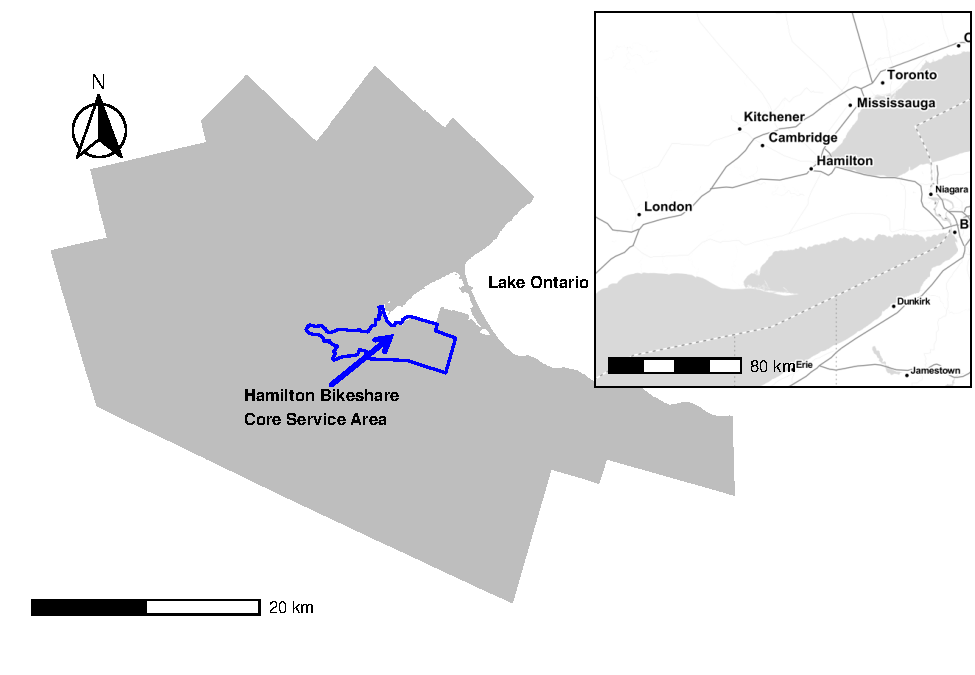
\includegraphics[width=0.9\linewidth]{Bike-share-spatial-equity_files/figure-latex/hamilton-and-sobi-service-area-1} 

}

\caption{The core service area of Hamilton Bike Share is outlined in black. Hamilton Census Metropolitan Area is shown in grey.}\label{fig:hamilton-and-sobi-service-area}
\end{figure}

\begin{figure}

{\centering 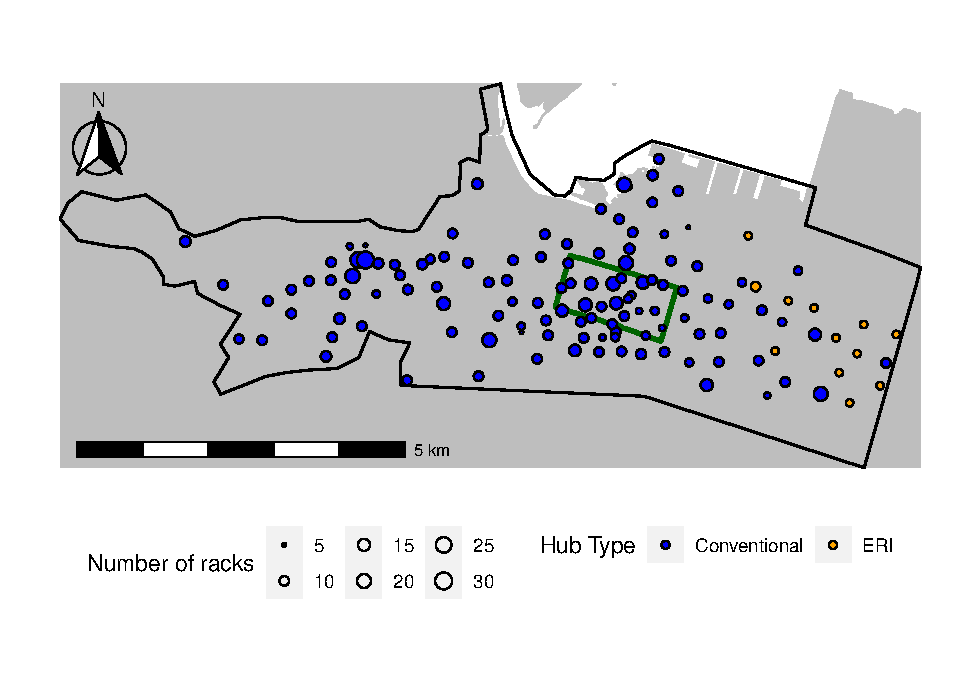
\includegraphics[width=1\linewidth]{Bike-share-spatial-equity_files/figure-latex/sobi-stations-in-hamilton-1} 

}

\caption{The spatial distribution of bicycle share stations in Hamilton, Ontario. The service area of Hamilton Bike Share is outlined in black and the city's downtown core is outlined in pink. Hamilton Census Metropolitan Area is shown in grey.}\label{fig:sobi-stations-in-hamilton}
\end{figure}

\hypertarget{sec:methods}{%
\section{4. Methods and Data}\label{sec:methods}}

\hypertarget{floating-catchment-area}{%
\subsection{4.1. Floating Catchment
Area}\label{floating-catchment-area}}

Floating catchment area (FCA) methods are an approach commonly used in
the healthcare accessibility literature. This approach is more
appropriate and informative than calculating provider-to-population
ratios (PPR) that simply divide the level of supply of a service (e.g.,
the number of bicycle racks at a station) by the population who have
access to the service (Paez et al., 2019). In particular, the Two-Step
Floating Catchment Area (2SFCA) method (Luo and Wang, 2003; Radke and
Mu, 2000) produces flexible catchment areas instead of using rigid
boundaries like PPR. This provides more useful information because it
does not assume that people are limited to service within pre-defined
boundaries (Paez et al., 2019). This is an important property that
supports our rationale for applying this method to measure accessibility
to Hamilton Bike Share. The City of Hamilton has positioned stations
between 300 and 600 m apart, but anticipates that hubs will service
those living within a 250 m buffer from the station (Hamilton, 2015b).
The latter constitutes a normative statement: people ought to be able to
access a station in less than 600 m if they live in the core service
area, with usage coming from 250 m around. However, it is not known how
far people are actually willing to travel to reach a station. It would
be reasonable to assume that people are willing to walk beyond this
threshold to access other stations if the ones nearest them have no
supply of bicycles.

More recently, the \emph{balanced} floating catchment area approach was
developed to address issues with demand and supply inflation that result
from the overlapping catchment areas produced by earlier FCA methods
(Paez et al., 2019). Briefly, overlapping catchment areas lead to
inflation of population totals and deflation of service levels across a
study area and generates inaccurate or misleading accessibility
estimates. In contrast, Paez et al.~(2019) adjusted the impedance
weights so that both supply and demand are proportionally allocated. The
result is a FCA method that balances the population and level of service
by eliminating the over-counting of population and level of service that
leads to distortions in demand and supply. Other benefits of this
adjusted method include consideration of competition which can occur
when catchment areas overlap, as well as the preservation of population
and level of service. Balanced floating catchment area methods have been
used to explore accessibility to health care providers (Paez et al.,
2019) and COVID-19 health care services (Pereira, Carlos Kauê Vieira
Braga, et al., 2021), but have not yet been used in the cycling
literature to explore issues of accessibility.

The first step in the floating catchment area method is to allocate the
population to be serviced by each Hamilton Bike Share station: \[
P_j = {\sum_{i = 1}^{n} P_i{w_{ij}}}
\]

As seen in the equation above, the population allocated to station \(j\)
is the weighted sum of the population in the region; a spatial weight
\(w_{ij}\) represents the friction that the population at \(i\) faces
when reaching station \(j\), and is usually given by a distance-decay
function, so that each station is assumed to service only a segment of
the population within a limited geographical range.

Next, the supply at each station (i.e., the maximum number of bicycle
racks) is divided by its estimated service population within the
established catchment area; this gives the level of service of station
\(j\) in bicycle racks per person: \[
L_j = \frac {S_j}{P_j} = \frac {S_j}{{\sum_{i = 1}^{n} P_i{w_{ij}}}}
\]

Finally, the accessibility of population cell \(i\) is calculated as the
weighted sum of the level of service of all stations that can be reached
from there according to the spatial weights: \[
A_i = {\sum_{j = 1}^{J} L_j{w_{ji}}} = {\sum_{j = 1}^{J} \frac {S_j{w_{ji}}}{\sum_{i = 1}^{n} P_i{w_{ij}}}}
\]

The balanced approach of Paez et al (2019) replaces the spatial weights
with normalized versions as follows: \[
{w_{ij}^{i} = \frac {w_{ij}}{\sum_{j = 1}^{J} {w_{ji}}}}
\]

\noindent and: \[
{w_{ij}^{j} = \frac {w_{ij}}{\sum_{j = 1}^{J} {w_{ji}}}}
\]

These weights satisfy the following properties: \[
\sum_{j = 1}^{J} {w^i_{ji}} = 1
\]

\noindent and: \[
\sum_{i = 1}^{n} {w^j_{ji}} = 1
\]

With these weights, accessibility can be calculated without risk of
demand or supply inflation: \[
A_i = {\sum_{j = 1}^{J} \frac {S_j{w^j_{ij}}}{\sum_{i = 1}^{n} P_i{w^i_{ij}}}}
\]

By allocating the population and level of service proportionally, this
method preserves the values of the population and level of service and
provides a regional provider-to-population ratio since: \[
\sum_{i=1}^n A_i = \sum_{j=1}^J L_j = \frac{\sum_{j=1}^JS_j}{\sum_{i=1}^n P_i}
\]

In fact, since the proportional allocation procedure means that any
proportion of the population allocated to a station is never allocated
to other stations, and conversely any level of service allocated to a
population is never re-allocated elsewhere, this property is replicated
for any level of aggregation. For this paper, we employ a hybrid
location-based and person-based approach to calculating accessibility
using disaggregated population data. In their review of accessibility
measures, Geurs and van Wee (2004) highlight the need for greater
inclusion of individual spatio-temporal constraints but acknowledge the
challenges of acquiring and analyzing person-based data. This comes
after Kwan's (1998) work to show that space-time measures are better
able of capturing interpersonal differences, especially the effect of
space-time constraints on individual behaviour, and are more helpful for
unraveling gender/ethnic differences. Applying the balanced floating
catchment area approach allows us to examine accessibility by
stratifying according to median total household income, which
constitutes the individual component of the accessibility measure (Geurs
and van Wee, 2004). However, conducting a further sensitivity analysis
to measure accessibility at different walking time thresholds would help
to consider potential spatio-temporal constraints. Different people may
be willing to travel different distances to access a public bicycle
share station.

\hypertarget{pycnophylactic-interpolation}{%
\subsection{4.2. Pycnophylactic
Interpolation}\label{pycnophylactic-interpolation}}

To obtain population at sub-census geography levels (at the micro
scale), we use pycnophylactic interpolation (Tobler, 1979). We obtained
population data from the 2016 Census of Canada for dissemination areas
(DA), which is the smallest publicly available census geography in
Canada. These zonal values of the population were interpolated to
smaller polygons 50-by-50 m in size. Pycnophylactic interpolation
involves smoothing out the population from each dissemination area while
preserving total volume {[}see Figure \ref{fig:da-population}{]}. When
interpolating the population at this high level of resolution, it is
important to ensure that population numbers were not allocated to areas
where people do not live in Hamilton (for example, to parks, large
institutional buildings, etc.). To do so, we retrieved shapefiles for
various geographic features {[}see Table \ref{tab:data-features}{]} from
Open Hamilton. Next, we removed these features from the PBSP core
service area and used pycnophylactic interpolation to disaggregate and
reallocate population within the remaining area {[}see Figure
\ref{fig:interpolated-population}{]}.

\begin{table}

\caption{\label{tab:data-features}\label{tab:landscape-features}Landscape features extracted from the Hamilton Bike Share core service area before population is interpolated.}
\centering
\resizebox{\linewidth}{!}{
\begin{tabular}[t]{>{}l|>{\raggedright\arraybackslash}p{30em}}
\toprule
Feature & Description\\
\midrule
\cellcolor{gray!6}{\textbf{Hamilton Bike Share Stations}} & \cellcolor{gray!6}{The location of stations and the number of racks available at each station.}\\
\textbf{Golf Courses} & The location of City and privately owned golf courses.\\
\cellcolor{gray!6}{\textbf{Parks}} & \cellcolor{gray!6}{The location of parks and other green spaces.}\\
\textbf{Designated Large Employment Areas} & The location of large business parks and industrial lands.\\
\cellcolor{gray!6}{\textbf{Municipal Parking Lots}} & \cellcolor{gray!6}{The location of municipal car parks.}\\
\addlinespace
\textbf{Cemeteries} & The location of cemeteries.\\
\cellcolor{gray!6}{\textbf{Environmentally Sensitive Areas}} & \cellcolor{gray!6}{The location of either land or water areas containing natural features or significant ecological functions.}\\
\textbf{Streets} & The street network in Hamilton, including road classification for highways.\\
\cellcolor{gray!6}{\textbf{Educational Institutions}} & \cellcolor{gray!6}{The location of all educational institutions and schools.}\\
\textbf{Places of Worship} & The location of buildings used for religious congregations.\\
\addlinespace
\cellcolor{gray!6}{\textbf{Municipal Service Centers}} & \cellcolor{gray!6}{The location of all municipal service centers, including City Hall.}\\
\textbf{Recreation and Community Centers} & The location of all recreation and community centers.\\
\cellcolor{gray!6}{\textbf{Arenas}} & \cellcolor{gray!6}{The location of all indoor arenas.}\\
\textbf{Emergency Stations} & The location of all Emergency Management Services (EMS) Ambulance stations.\\
\cellcolor{gray!6}{\textbf{Fire Stations}} & \cellcolor{gray!6}{The location of all fire stations.}\\
\addlinespace
\textbf{Police Stations} & The location of all police stations.\\
\cellcolor{gray!6}{\textbf{Railways}} & \cellcolor{gray!6}{The railway network in Hamilton.}\\
\textbf{Hospitals} & The location of all hospitals.\\
\bottomrule
\end{tabular}}
\end{table}

\begin{figure}

{\centering 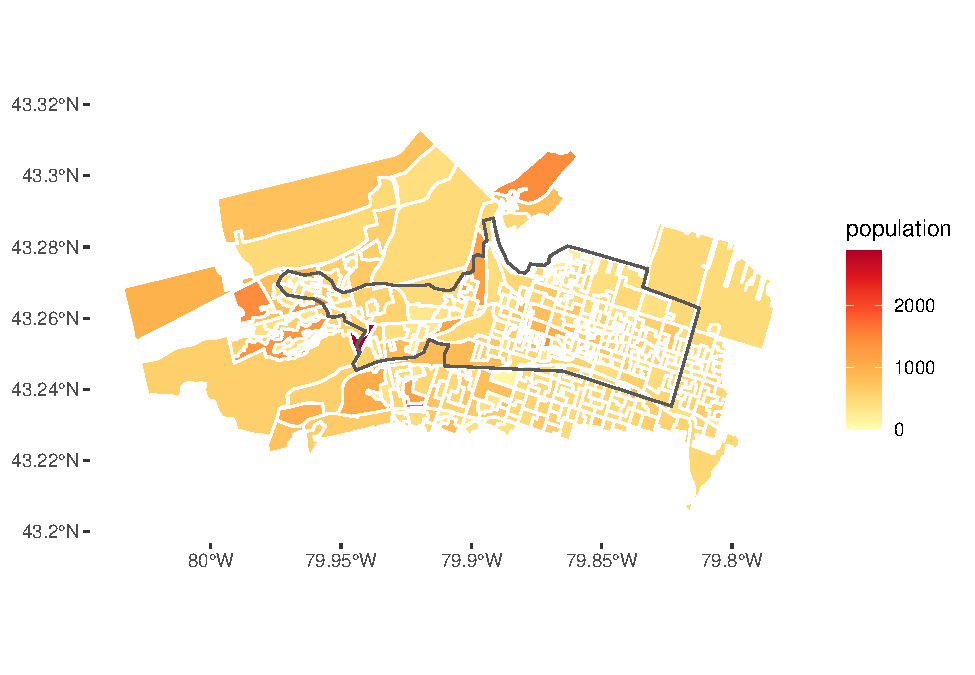
\includegraphics[width=0.9\linewidth]{Bike-share-spatial-equity_files/figure-latex/da-population-1} 

}

\caption{Population in all dissemination areas (outlined in white) that are inside or touch the bounding box of the Hamilton Bike Share core service area (outlined in black).}\label{fig:da-population}
\end{figure}

\begin{figure}

{\centering 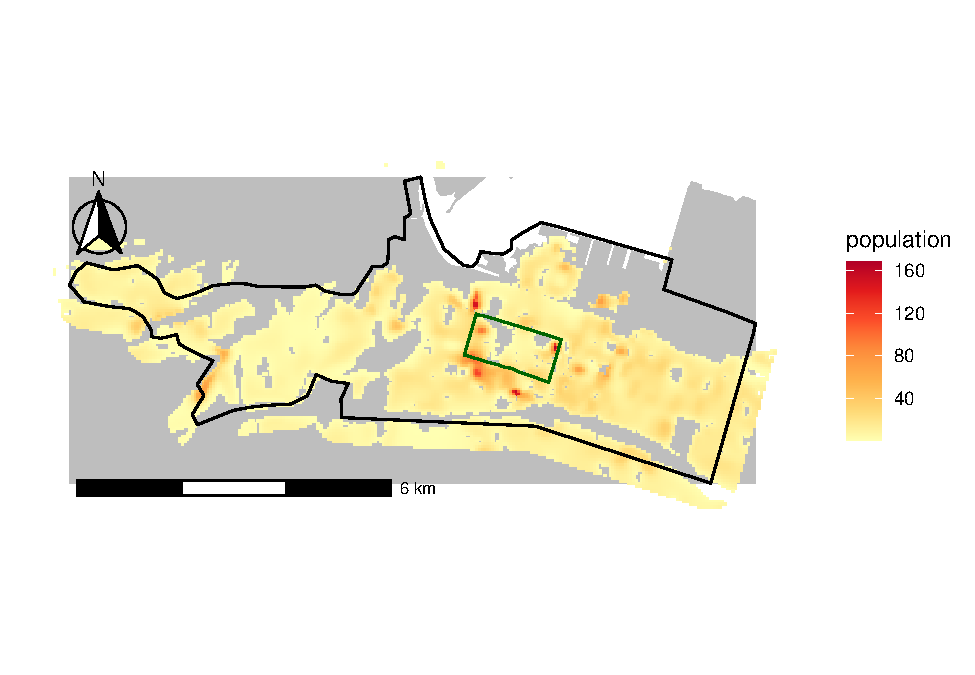
\includegraphics[width=0.9\linewidth]{Bike-share-spatial-equity_files/figure-latex/interpolated-population-1} 

}

\caption{Interpolated population in the Hamilton Bike Share's core service area (outlined in black) and within 30 minutes of walking to the core service area. Each population cell is 50-by-50 m in size. The downtown area is outlined in dark green.}\label{fig:interpolated-population}
\end{figure}

\hypertarget{travel-time-matrix}{%
\subsection{4.3. Travel Time Matrix}\label{travel-time-matrix}}

To calculate walking times from the centroid of our micro population
cells, we extracted OpenStreetMap data for Hamilton Bike Share's service
area from \href{https://download.bbbike.org/osm/bbbike/}{BBBike}, an
online cycle route planner that interfaces with OpenStreetMap.
OpenStreetMap data provides the networks for calculating walking times
from each population cell to nearby bicycle share stations, using a
maximum walking distance of 10 km and walking time of 30 minutes as
thresholds. A travel time matrix was created with the origins as the
coordinates of the population cells and the destinations as the
coordinates of the bicycle share stations within the maximum threshold.
This process provides a more realistic measure of the friction of
reaching stations by taking infrastructure into account of travel times,
rather than using the Euclidean distance from population cell to
station. Routing and travel time calculations were completed using the
\texttt{R} package \texttt{r5r}, used for rapid realistic routing
operations (Pereira, Saraiva, et al., 2021).

\hypertarget{data}{%
\subsection{4.4. Data}\label{data}}

All data for this research were accessed from publicly available Census
of Canada sources, from OpenStreetMaps, and from Open Hamilton\footnote{https://open.hamilton.ca/},
a public online repository of data curated by the City of Hamilton.

\hypertarget{results}{%
\section{5. Results}\label{results}}

\hypertarget{accessibility-by-distance-thresholds}{%
\subsection{5.1. Accessibility by Distance
Thresholds}\label{accessibility-by-distance-thresholds}}

Consensus regarding the distance that individuals are willing to walk to
access a bicycle share station is lacking, but the literature on walking
behaviour can provide some guidelines to determine the thresholds for
sensitivity analysis. Previous studies have found that living within 250
m (Fuller et al., 2011) and 300 m (Kabra et al., 2020) is correlated
with bike share use, while other research has found that walking trips
are less than 600 m and rarely more than 1200 m (Millward et al., 2013)
or a median distance of 650 m (Larsen et al., 2010). In Hamilton,
Hamilton Bike Share will depict a map at some stations to show the user
the locations of the other nearest stations within a five minute walk,
which suggests that this is an average distance that people are expected
to walk. National Association of City Transportation Officials (NACTO)
has a similar normative guide (City Transportation Officials, 2015).

In the present case, we found that congested accessibility calculated
using the balanced FCA approach increases with a threshold between two
and four minutes, but is then maximized at 5 minutes. Accessibility
decreases substantially after eight minutes, which is intuitive given
that demand on a limited supply increases as more people can reach each
station.

For this reason, we experiment with various thresholds by conducting a
sensitivity analysis to calculate accessibility at different walking
times from population cell to bicycle share station: 3 minutes, 5
minutes, 10 minutes, and 15 minutes. We categorize these thresholds as
minimum, average, maximum, and extreme, respectively. At each threshold,
we compare accessibility between the current system and the original
system to examine the contribution of the additional equity stations.
When considering the results reported below, it is important to remember
that accessibility is technically a form of smoothing (O'Kelly and
Horner, 2003, pp. 7--8): smaller thresholds produce less smoothing
(which can result in ``spiky'' accessibility landscapes), while larger
thresholds produce more smoothing and fewer spikes.

\hypertarget{minimum-threshold}{%
\subsubsection{5.1.1. Minimum Threshold}\label{minimum-threshold}}

With a walking distance of three minutes, we find that there are 25.2
bicycle racks per person system-wide in the original system
configuration (i.e., without equity stations). The addition of equity
stations increases this ratio slightly to 25.4 bicycles per person.
Figure \ref{fig:figure-6} presents a comparison of accessibility between
the systems for the population cells. Accessibility is fairly uniform
overall, with the exception of two small areas where accessibility is
slightly higher. This high level of system-wide accessibility occurs
because the population that can reach bicycle share stations when travel
time is 3 minutes or less is very limited, and accessibility is strongly
shaped by a few locations that concentrate population and stations.

\begin{figure}

{\centering 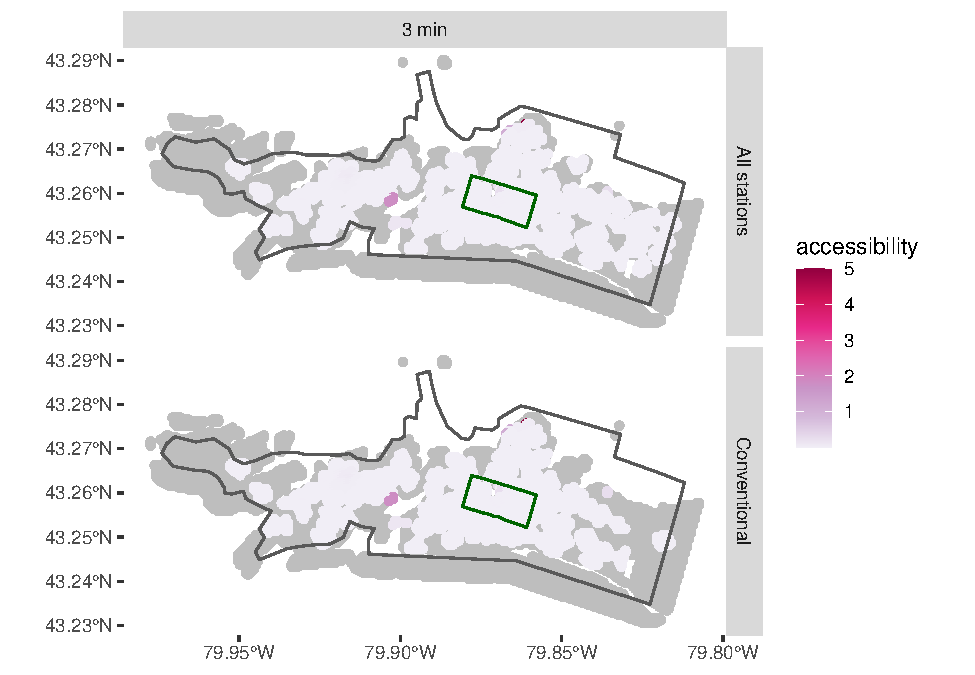
\includegraphics[width=0.9\linewidth]{Bike-share-spatial-equity_files/figure-latex/figure-6-1} 

}

\caption{Accessibility at 3 minutes walk (minimum threshold) compared between current system with equity stations and the original system without equity stations.}\label{fig:figure-6}
\end{figure}

\hypertarget{average-threshold}{%
\subsubsection{5.1.2. Average Threshold}\label{average-threshold}}

With a walking distance of five minutes, we find that there are 68.6
bicycle racks per person system-wide in the original system
configuration (i.e., without equity stations). With the addition of
equity stations, there are now 68.8 bicycle racks per person. At this
threshold, there are more bicycle racks per person than at the minimum
threshold. System-wide accessibility has in fact increased: the
population that can reach the stations has grown, but not to the the
point that congestion effects begin to take place. Figure
\ref{fig:figure-7} presents a comparison of accessibility between the
systems. Again, accessibility is fairly uniform, with the exception of
one very small area.

\begin{figure}

{\centering 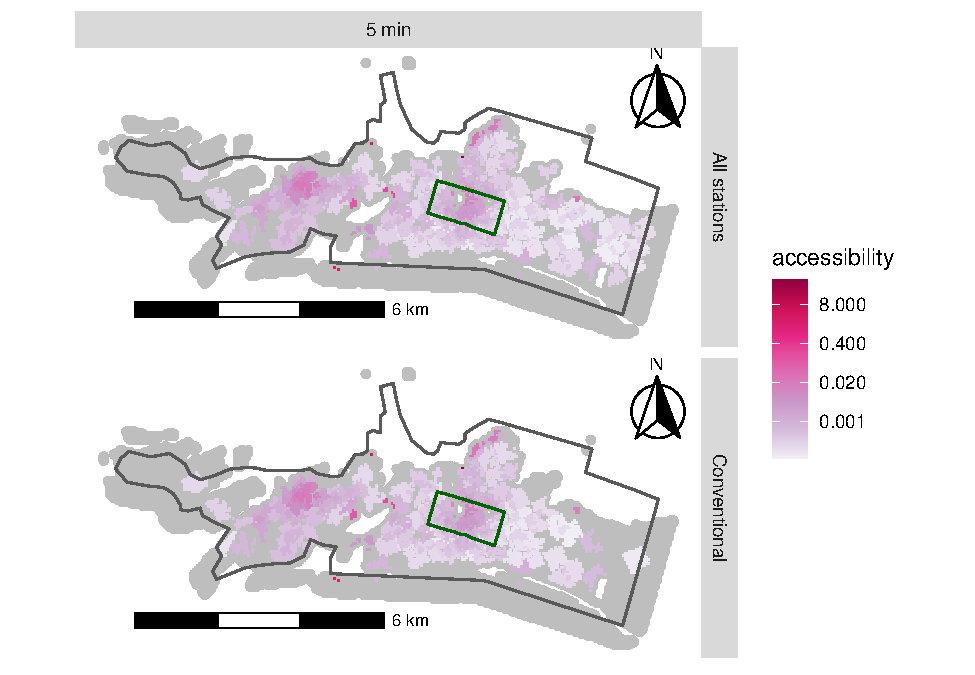
\includegraphics[width=0.9\linewidth]{Bike-share-spatial-equity_files/figure-latex/figure-7-1} 

}

\caption{Accessibility at 5 minutes walk (average threshold) compared between current system with equity stations and the original system without equity stations.}\label{fig:figure-7}
\end{figure}

\hypertarget{maximum-threshold}{%
\subsubsection{5.1.3. Maximum Threshold}\label{maximum-threshold}}

With a walking distance of ten minutes, we find that there are 3.61
bicycle racks per person system-wide in the original system
configuration (i.e., without equity stations). With the addition of
equity stations, there are now 3.74 bicycles per person. Figure
\ref{fig:figure-8} presents a comparison of accessibility between the
systems. Differences in accessibility across the service area are now
apparent, with users near the university and its adjacent neighborhoods,
as well as neighborhoods north of the downtown area (the latter is
outlined in green), having slightly higher accessibility. While the
differences are modest, they are more apparent at this threshold than at
shorter walking distances.

\begin{figure}

{\centering 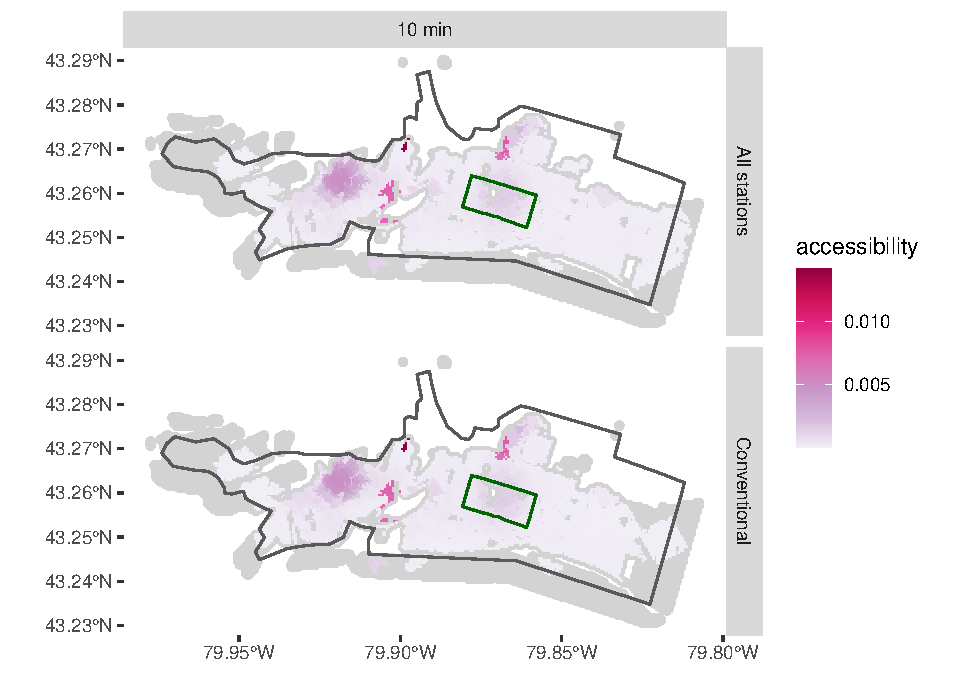
\includegraphics[width=0.9\linewidth]{Bike-share-spatial-equity_files/figure-latex/figure-8-1} 

}

\caption{Accessibility at 10 minutes walk (maximum threshold) compared between current system with equity stations and the original system without equity stations.}\label{fig:figure-8}
\end{figure}

\hypertarget{extreme-threshold}{%
\subsubsection{5.1.4. Extreme Threshold}\label{extreme-threshold}}

With a walking distance of fifteen minutes, we find that there are 2.44
bicycle racks per person system-wide in the original system
configuration (i.e., without equity stations). With the addition of
equity stations, there are now 2.55 bicycles per person. Figure
\ref{fig:figure-9} presents a comparison of accessibility between the
systems. Users near the university and the neighborhoods north of the
downtown area (the latter is outlined in green) have the highest
accessibility, followed by those who live in the city's downtown area.
Accessibility in the east end, where equity stations were implemented,
of the core service area remains low.

\begin{figure}

{\centering 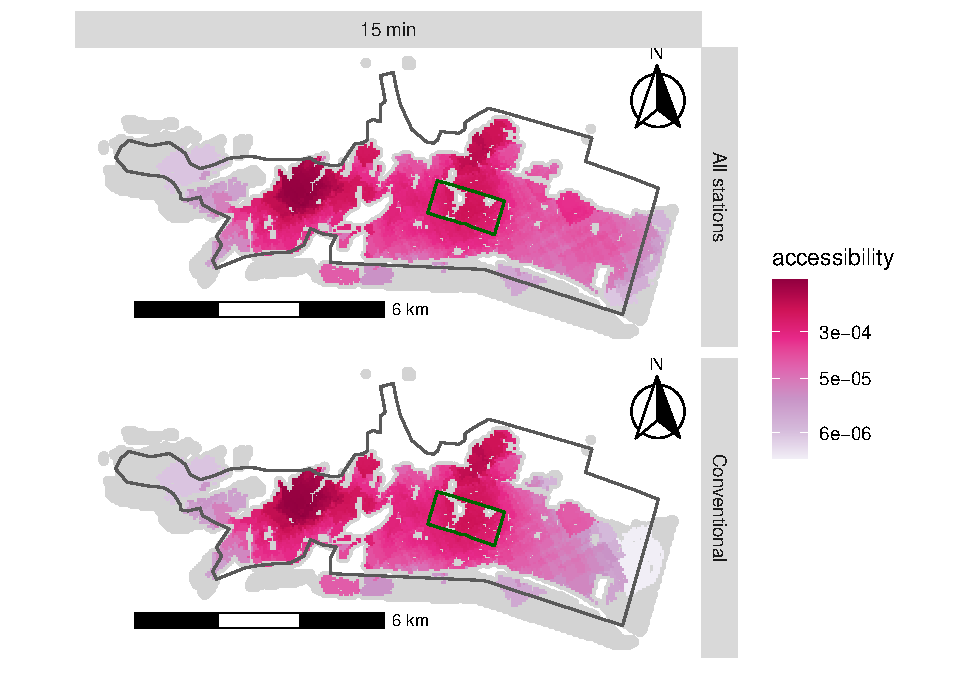
\includegraphics[width=0.9\linewidth]{Bike-share-spatial-equity_files/figure-latex/figure-9-1} 

}

\caption{Accessibility at 15 minutes walk (extreme threshold) compared between current system with equity stations and the original system without equity stations.}\label{fig:figure-9}
\end{figure}

\hypertarget{accessibility-by-median-total-household-income}{%
\subsection{5.2. Accessibility by Median Total Household
Income}\label{accessibility-by-median-total-household-income}}

A unique property of the balanced floating catchment area method is that
data can be reaggregated while preserving the total population in the
service area and the supply at each station. This avoids demand and
supply inflation, and also enables us to present findings in a way that
is perhaps more intuitive to interpret. Therefore, we reaggregate
population and accessibility from the 50-by-50 m population cells to the
dissemination area. We then can compare accessibility to median total
household income statistics from the Canadian census results from 2016.

Figures 1 {[}\ref{fig:figure-bi-map-threshold-3}{]}, 2
{[}\ref{fig:figure-bi-map-threshold-5}{]}, 3
{[}\ref{fig:figure-bi-map-threshold-10}{]}, and 4
{[}\ref{fig:figure-bi-map-threshold-15}{]} depict bivariate choropleth
maps that combine the spatial distribution of accessibility and median
total household income, using tertiles for the coloring scheme. In each
figure, the top panel is the system without the equity stations (i.e.,
the original system configuration), and the bottom panel is
accessibility in the current system with equity stations. As expected,
the analysis indicates that the extreme threshold of fifteen minutes is
associated with the largest number of people who are within the assumed
service area of stations. We find that stations added to Hamilton's
public bicycle share program did indeed expand the spatial coverage of
the system, leading to more balance across the service area. By
implementing equity stations in areas with lower median total household
income in Hamilton, the PBSP attained greater horizontal equity by
extending the spatial distribution of bicycles across the city. This is
particularly evident at the minimum and average thresholds of three and
five minutes, respectively, where the equity stations fill a number of
gaps in program coverage.

\begin{figure}
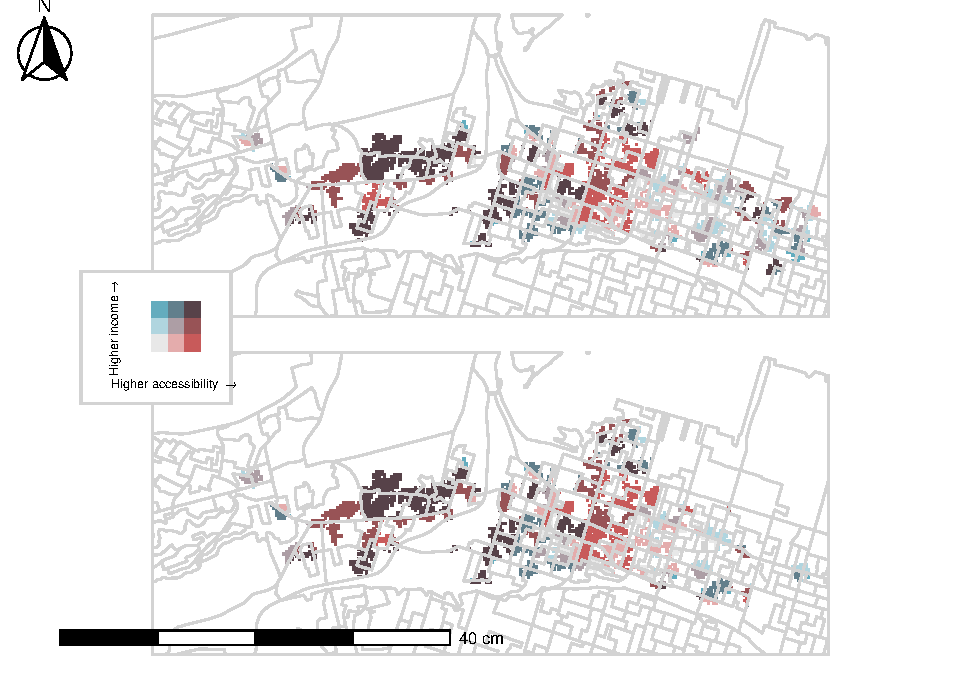
\includegraphics[width=1\linewidth]{Bike-share-spatial-equity_files/figure-latex/figure-bi-map-threshold-3-1} \caption{\label{fig-bivariate-map-threshold-3}Bivariate map of accessibility and income (threshold: 3 min): without equity stations (top panel) and with equity stations (bottom panel)}\label{fig:figure-bi-map-threshold-3}
\end{figure}

\begin{figure}
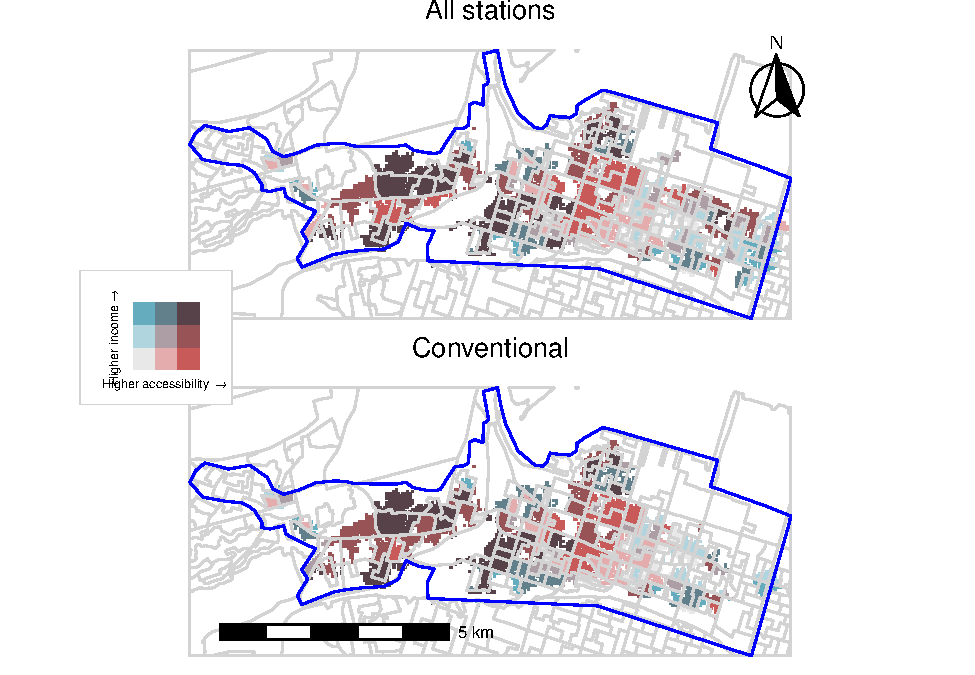
\includegraphics[width=1\linewidth]{Bike-share-spatial-equity_files/figure-latex/figure-bi-map-threshold-5-1} \caption{\label{fig-bivariate-map-threshold-5}Bivariate map of accessibility and income (threshold: 5 min): without equity stations (top panel) and with equity stations (bottom panel)}\label{fig:figure-bi-map-threshold-5}
\end{figure}

\begin{figure}
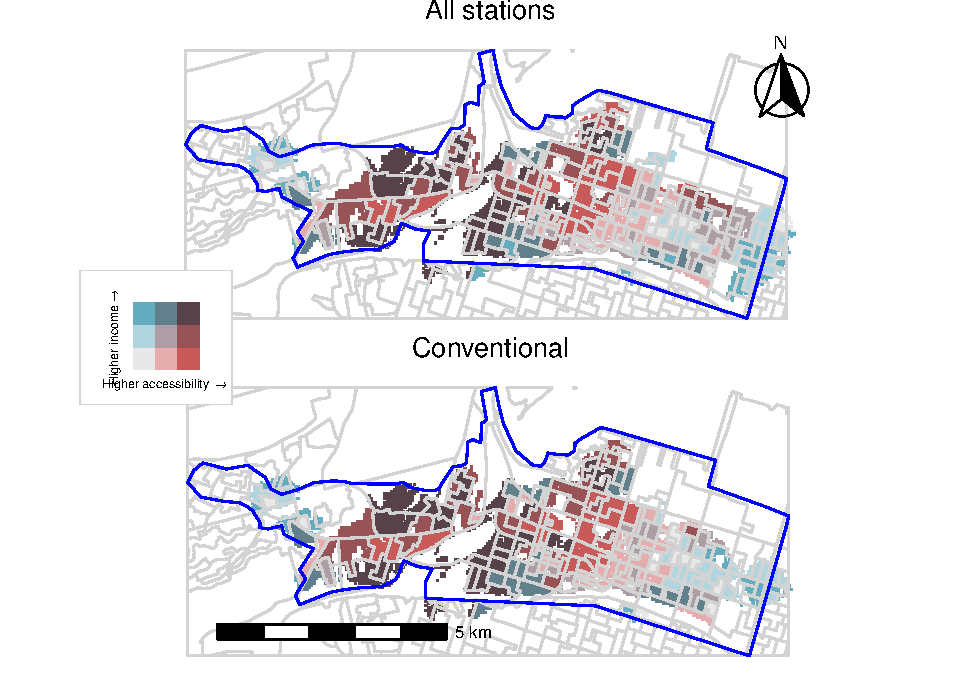
\includegraphics[width=1\linewidth]{Bike-share-spatial-equity_files/figure-latex/figure-bi-map-threshold-10-1} \caption{\label{fig-bivariate-map-threshold-10}Bivariate map of accessibility and income (threshold: 10 min): without equity stations (top panel) and with equity stations (bottom panel)}\label{fig:figure-bi-map-threshold-10}
\end{figure}

\begin{figure}
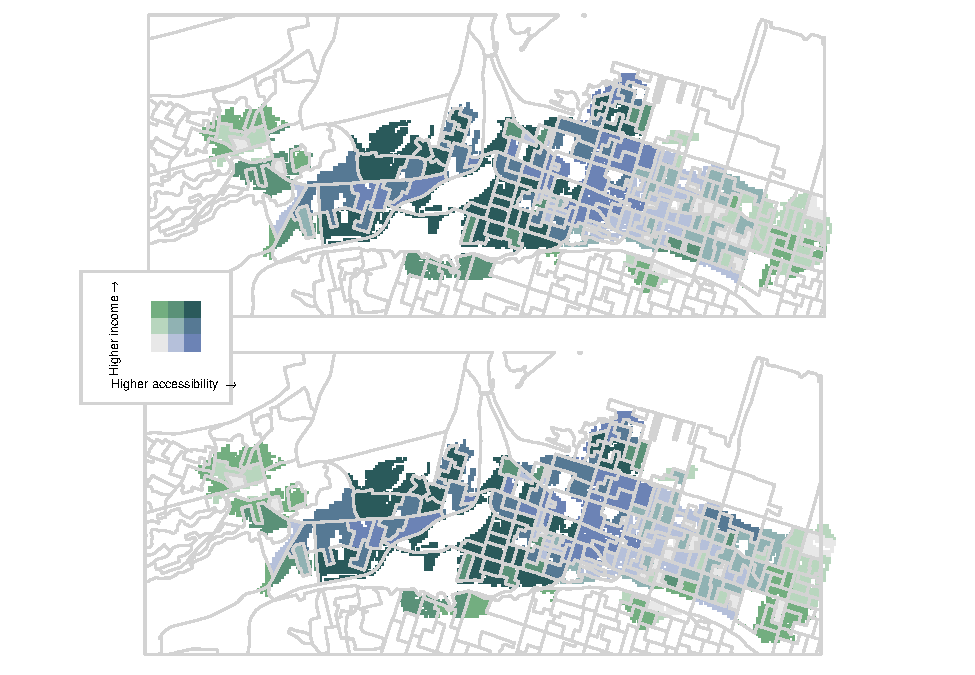
\includegraphics[width=1\linewidth]{Bike-share-spatial-equity_files/figure-latex/figure-bi-map-threshold-15-1} \caption{\label{fig-bivariate-map-threshold-15}Bivariate map of accessibility and income (threshold: 15 min): without equity stations (top panel) and equity stations (bottom panel)}\label{fig:figure-bi-map-threshold-15}
\end{figure}

To further explore this issue and examine vertical equity, we aggregate
accessibility by median total household income across all geographies
(see Table \ref{tab:accessibility-income}). Similar to Hosford and
Winters (2018), we find that Hamilton's PBSP already serviced a large
proportion of the population in the bottom and second quintiles of
median total household income. This may well be an artifact of the
spatial socioeconomic and demographic profile of Hamilton, where the
most dense parts of the city (where a PBSP is most easily launched) are
also those with relatively lower incomes. On the other hand, the levels
of accessibility to Hamilton's PBSP are generally lower for populations
in the bottom 20\% of median total household income, compared to
populations in the top 20\%.

The spatial mapping reveals that the addition of equity stations
increased horizontal equity by growing the population serviced
irrespective of the walking threshold. The largest gains were made for
dissemination areas in the second 20\%, where an additional 3,073 and
5,395 people could reach a bicycle share station within three and five
minutes walk, respectively, after the addition of equity stations.
However, we find that there were only small increases in the population
in the bottom 20\% of median total household income who are serviced by
the equity stations, and the accessibility gains are also quite modest
and smaller than for populations in the second and third quintiles of
median total household income. This suggests that income disparities
persist, albeit this depends on the walking time thresholds. With and
without equity stations, people in the top 20\% of income have the
highest level of access at a threshold of ten and fifteen minutes.
Although dissemination areas in the second 20\% have the highest level
of access by a significant amount at lower distance thresholds, the
bottom 20\%, who may benefit the most from Hamilton Bike Share's equity
initiatives, have the lowest access at three minutes threshold and the
second lowest access at all other thresholds.

\begin{table}

\caption{\label{tab:accessibility-income}\label{tab:accessibility-by-income}Accessibility and population serviced by income quintile and between systems (with and without equity stations). Total population is the population by income quintile in the DAs that have any PBSP service at all.}
\centering
\resizebox{\linewidth}{!}{
\begin{tabular}[t]{lccccccl}
\toprule
\multicolumn{2}{c}{ } & \multicolumn{2}{c}{Without Equity Stations} & \multicolumn{2}{c}{With Equity Stations} & \multicolumn{2}{c}{Difference} \\
\cmidrule(l{3pt}r{3pt}){3-4} \cmidrule(l{3pt}r{3pt}){5-6} \cmidrule(l{3pt}r{3pt}){7-8}
Income Quintile & Total Population & Population & Accessibility & Population & Accessibility & Population & Accessibility\\
\midrule
\addlinespace[0.3em]
\multicolumn{8}{l}{\textbf{Threshold - 3 minutes}}\\
\hspace{1em}\cellcolor{gray!6}{Bottom 20\%} & \cellcolor{gray!6}{43441} & \cellcolor{gray!6}{22359} & \cellcolor{gray!6}{2.377} & \cellcolor{gray!6}{22798} & \cellcolor{gray!6}{2.424} & \cellcolor{gray!6}{439} & \cellcolor{gray!6}{0.047}\\
\hspace{1em}Second 20\% & 33312 & 9347 & 12.203 & 12420 & 12.281 & 3073 & 0.078\\
\hspace{1em}\cellcolor{gray!6}{Third 20\%} & \cellcolor{gray!6}{30940} & \cellcolor{gray!6}{7745} & \cellcolor{gray!6}{3.093} & \cellcolor{gray!6}{9455} & \cellcolor{gray!6}{3.156} & \cellcolor{gray!6}{1710} & \cellcolor{gray!6}{0.063}\\
\hspace{1em}Fourth 20\% & 20185 & 1673 & 4.119 & 1673 & 4.119 & 0 & 0.000\\
\hspace{1em}\cellcolor{gray!6}{Top 20\%} & \cellcolor{gray!6}{27541} & \cellcolor{gray!6}{2114} & \cellcolor{gray!6}{3.408} & \cellcolor{gray!6}{2379} & \cellcolor{gray!6}{3.434} & \cellcolor{gray!6}{265} & \cellcolor{gray!6}{0.026}\\
\addlinespace[0.3em]
\multicolumn{8}{l}{\textbf{Threshold - 5 minutes}}\\
\hspace{1em}Bottom 20\% & 43441 & 35477 & 1.302 & 35803 & 1.357 & 326 & 0.055\\
\hspace{1em}\cellcolor{gray!6}{Second 20\%} & \cellcolor{gray!6}{33312} & \cellcolor{gray!6}{17513} & \cellcolor{gray!6}{56.048} & \cellcolor{gray!6}{22908} & \cellcolor{gray!6}{56.137} & \cellcolor{gray!6}{5395} & \cellcolor{gray!6}{0.089}\\
\hspace{1em}Third 20\% & 30940 & 15117 & 4.258 & 18309 & 4.291 & 3192 & 0.033\\
\hspace{1em}\cellcolor{gray!6}{Fourth 20\%} & \cellcolor{gray!6}{20185} & \cellcolor{gray!6}{2867} & \cellcolor{gray!6}{1.094} & \cellcolor{gray!6}{3116} & \cellcolor{gray!6}{1.095} & \cellcolor{gray!6}{249} & \cellcolor{gray!6}{0.001}\\
\hspace{1em}Top 20\% & 27541 & 4052 & 5.925 & 4518 & 5.933 & 466 & 0.008\\
\addlinespace[0.3em]
\multicolumn{8}{l}{\textbf{Threshold - 10 minutes}}\\
\hspace{1em}\cellcolor{gray!6}{Bottom 20\%} & \cellcolor{gray!6}{43441} & \cellcolor{gray!6}{41824} & \cellcolor{gray!6}{0.603} & \cellcolor{gray!6}{41981} & \cellcolor{gray!6}{0.621} & \cellcolor{gray!6}{157} & \cellcolor{gray!6}{0.018}\\
\hspace{1em}Second 20\% & 33312 & 27546 & 0.860 & 30503 & 0.927 & 2957 & 0.067\\
\hspace{1em}\cellcolor{gray!6}{Third 20\%} & \cellcolor{gray!6}{30940} & \cellcolor{gray!6}{22394} & \cellcolor{gray!6}{0.772} & \cellcolor{gray!6}{25128} & \cellcolor{gray!6}{0.799} & \cellcolor{gray!6}{2734} & \cellcolor{gray!6}{0.027}\\
\hspace{1em}Fourth 20\% & 20185 & 4544 & 0.225 & 4989 & 0.227 & 445 & 0.002\\
\hspace{1em}\cellcolor{gray!6}{Top 20\%} & \cellcolor{gray!6}{27541} & \cellcolor{gray!6}{7989} & \cellcolor{gray!6}{1.160} & \cellcolor{gray!6}{9078} & \cellcolor{gray!6}{1.162} & \cellcolor{gray!6}{1089} & \cellcolor{gray!6}{0.002}\\
\addlinespace[0.3em]
\multicolumn{8}{l}{\textbf{Threshold - 15 minutes}}\\
\hspace{1em}Bottom 20\% & 43441 & 42208 & 0.534 & 42327 & 0.554 & 119 & 0.020\\
\hspace{1em}\cellcolor{gray!6}{Second 20\%} & \cellcolor{gray!6}{33312} & \cellcolor{gray!6}{30507} & \cellcolor{gray!6}{0.551} & \cellcolor{gray!6}{31069} & \cellcolor{gray!6}{0.611} & \cellcolor{gray!6}{562} & \cellcolor{gray!6}{0.060}\\
\hspace{1em}Third 20\% & 30940 & 26108 & 0.546 & 26660 & 0.573 & 552 & 0.027\\
\hspace{1em}\cellcolor{gray!6}{Fourth 20\%} & \cellcolor{gray!6}{20185} & \cellcolor{gray!6}{6312} & \cellcolor{gray!6}{0.093} & \cellcolor{gray!6}{7435} & \cellcolor{gray!6}{0.096} & \cellcolor{gray!6}{1123} & \cellcolor{gray!6}{0.003}\\
\hspace{1em}Top 20\% & 27541 & 10209 & 0.712 & 11089 & 0.714 & 880 & 0.002\\
\bottomrule
\multicolumn{8}{l}{\rule{0pt}{1em}\textit{Note: }}\\
\multicolumn{8}{l}{\rule{0pt}{1em} }\\
\multicolumn{8}{l}{\rule{0pt}{1em}\textsuperscript{a} With equity stations = Hamilton Bike Share current system (118 conventional stations, 12 equity stations)}\\
\multicolumn{8}{l}{\rule{0pt}{1em}\textsuperscript{b} Without equity stations = Hamilton Bike Share original system (118 conventional stations, no equity stations)}\\
\end{tabular}}
\end{table}

\hypertarget{discussion}{%
\section{6. Discussion}\label{discussion}}

Using disaggregated data in this paper, we examined spatial equity and
accessibility to Hamilton Bike Share, with a particular focus on
assessing the contribution of the program's equity stations. Use of a
balanced floating catchment area approach, combined with pycnophylactic
interpolation, enabled us to measure accessibility on a micro scale
which is a sensible approach to avoid the ``absorption of disparities'',
as articulated by Chen et al.~(2019). This differentiates our analysis
from similar papers exploring equity in PBSPs that use larger
geographical units of analysis or that focus on station location instead
of level of service. In this way, our paper has made contributions in a
positive way by applying an intuitive and useful approach to measure
accessibility to a PBSP, and in a normative way by serving to inform
future investments in cycle infrastructure for Hamilton Bike Share.

The sensitivity analysis revealed that accessibility to Hamilton Bike
Share stations is maximized at five minutes and decreases significantly
by eight minutes {[}see Table \ref{tab:accessibility-income}{]}. This
reflects the normative guide advertised on some bicycle share stations
in Hamilton showing other stations within a five minute walk, as well as
the directive of NACTO (City Transportation Officials, 2015). We find
that over 118,000 people can access a bicycle share station within a 15
minute walk, which represents roughly 85\% of the total population in
the core service area {[}see Table \ref{tab:accessibility-income}{]}. At
a minimum threshold of three minutes, too few people can reach stations
which leads to relatively high levels of service since there is little
crowding. However, accessibility is at its lowest after eight minutes
whereby congestion effects due to increased potential demand kick in.
The City of Hamilton has recognized from the launch of the PBSP that
substantially more stations and bicycles are needed to service the area
(Hamilton, 2015b). With a service area of 40 sq.km, it is estimated that
Hamilton should have between 380 and 440 stations instead of 130, and
1,500 bicycles instead of 900 (Hamilton, 2015b). Reduced capacity within
the system leads to gaps in coverage in some areas of the city ``with
some areas not having the recommended station density of 300m between
stations or 10 stations per square km'' (Hamilton, 2015b). This study
illustrates the consequences of an imbalanced system whereby levels of
accessibility are not equitable across income groups.

We found that equity stations increased horizontal equity in Hamilton's
core service area. Figures \ref{fig:figure-bi-map-threshold-3},
\ref{fig:figure-bi-map-threshold-5},
\ref{fig:figure-bi-map-threshold-10}, and
\ref{fig:figure-bi-map-threshold-15} demonstrate how gaps in service
were filled by these additional stations. This indicates that more
individuals at all income quintiles can access Hamilton Bike Share,
which leads to a more balanced or equal program. In this respect, there
are some commonalities between the expansions of Hamilton Bike Share and
that of Citi Bike in New York. Babgoli et al.~(2019) found a slight but
not statistically significant increase in the proportion of
neighborhoods with the highest levels of poverty with stations after the
Citi Bike expansion in 2015. Although the Citi Bike expansion was not
specifically driven by a desire to reduce inequity in access, 16\% of
neighborhoods with the highest levels of poverty had stations compared
to 12\% before. Similarly, with the addition of equity stations, there
were large gains in accessibility for the second 20\% at the average
threshold, over 5,000 more people, but much smaller gains for the bottom
20\% with only 326 more people.

Vertical inequity, however, persisted as evidenced by differences in
accessibility according to income quintile. While the addition of equity
stations seems to modestly increase accessibility for all income groups
at all thresholds, they did not increase accessibility substantially for
any single income group. Most importantly, individuals in the bottom
20\% of median total household income have the second lowest level of
access to Hamilton Bike Share at most thresholds (average, maximum, and
extreme). At the minimum threshold, the bottom 20\% have the lowest
level of access. While previous research found that neighborhoods with
more disadvantage are better serviced by Hamilton Bike Share, the
authors used the Pampalon Deprivation Index to determine the level of
disadvantage for dissemination areas \emph{across} the city not just
within the core service area (Hosford and Winters, 2018). Instead, we
use median total household income for each dissemination area
\emph{within} the core service area. We conclude that Hamilton's PBSP,
while by default located in areas with more deprivation compared to
other cities, has disparities in accessibility between income groups.
With equity stations, many areas with low median total household income
in the east end of the service area continue to have low accessibility.
At the maximum and extreme thresholds, the top 20\% have the highest
level of access to Hamilton Bike Share. These findings aligns with other
studies from Tampa (Chen et al., 2019) and Seattle (Mooney et al.,
2019), which have found disparities in station location or access to
bicycles between levels of income and education.

Based on our analysis, we identified specific areas that have both low
accessibility and low median total household income which would benefit
from an increased supply of public bicycles. These empirical findings
provide support to the City of Hamilton's efforts to increase equity and
balance the system, and confirm that additional stations and bicycles
are needed to improve access not only for the bottom 20\% but for all
income groups. Figures \ref{fig:figure-bi-map-threshold-3},
\ref{fig:figure-bi-map-threshold-5},
\ref{fig:figure-bi-map-threshold-10}, and
\ref{fig:figure-bi-map-threshold-15} highlight potential locations for
new equity stations to better accommodate groups with lower
socioeconomic status.

\hypertarget{study-limitations}{%
\section{7. Study Limitations}\label{study-limitations}}

This paper did not examine or compare ridership data between
conventional and equity stations. Therefore, further research is needed
to determine whether the addition of equity stations encouraged more
cycling for low-income individuals living near them. Other studies have
specifically looked at differences in trip type, frequency, or length
among users from disadvantaged neighborhoods (Caspi and Noland, 2019;
Qian and Jaller, 2020; J. Wang and Lindsey, 2019a), but our analysis is
limited by the lack of publicly available route and individual user data
to conduct similar analyses for Hamilton Bike Share.

An additional limitation is the lack of publicly available information
about the number of bicycles at each station. Hamilton Bike share works
to balance the number of bicycles across stations, but it is reasonable
to expect that the number of bicycles will not match exactly the number
of racks at every station. Ideally, instead of number of bicycle racks
as our measure of supply, we would have liked to use the average number
of bicycles at stations, perhaps at different times during the day or
different seasons. Should this data become available, it would be
worthwhile to revisit the question to examine how well operation of the
system (including balancing of bicycles across stations) works to
maintain the nominal levels of accessibility examined in this paper.

\hypertarget{conclusion}{%
\section{8. Conclusion}\label{conclusion}}

The addition of specific equity stations to the public bicycle share
program in Hamilton, Ontario had the net effect of increasing
accessibility and reducing to some extent both horizontal and vertical
inequities. In particular, accessibility improved the most for those in
the second 20\% median total household income at all thresholds, but the
gains were only modest for all income groups. Dissemination areas with
the bottom 20\% had the lowest accessibility at three minutes, and
second lowest levels of accessibility at five, ten, and fifteen minutes.
Congestion effects were observed at higher thresholds, with
accessibility decreasing significantly once the catchment area is
increased to ten minutes walking.

Wang and Lindsey (2019b) have noted that there is a lack of research
that examines how bike share users' behaviour changes as a result of
program changes to station locations or improvements in accessibility.
As such, a logical next step to this research is to examine whether
Hamilton Bike Share's equity stations increased ridership or resulted in
new memberships in areas that were previously under-serviced. An
examination of the types of trips undertaken by residents in these areas
would also be informative, such as the study undertaken by Caspi and
Norland (2019) after bike share stations were implemented in low-income
Philadelphia neighborhoods. The bulk of cycling facilities that have
been built in Hamilton to date are located in the core service area near
the conventional stations. It would be worthwhile to explore the route
choice of bike share trips departing or ending at the equity stations
and to identify factors that specifically influence trips from these
stations, which would extend existing studies conducted by Scott and
colleagues (Lu et al., 2018; Scott and Ciuro, 2019; Scott et al., 2021).
This paper, combined with additional studies such as those
conceptualized above, would serve as a valuable case study for Hamilton
and other cities with PBSPs that wish to evaluate and address spatial
inequality in accessibility and transportation options in urban areas.

\hypertarget{acknowledgments}{%
\section{Acknowledgments}\label{acknowledgments}}

This research was completed using open software, and the authors wish to
acknowledge the developers of the following \texttt{R} packages:
\texttt{biscale} (Prener et al., 2020), \texttt{cowplot} (Wilke, 2020),
\texttt{data.table} (Dowle and Srinivasan, 2020), \texttt{disk.frame}
(ZJ, 2020), \texttt{gdistance} (van Etten, 2020), \texttt{gridExtra}
(Auguie, 2017), \texttt{kableExtra} (Zhu, 2020), \texttt{knitr} (Xie,
2020), \texttt{pycno} (Brunsdon, 2014), \texttt{r5r} (Saraiva et al.,
2020), \texttt{raster} (Hijmans, 2020), \texttt{rgdal} (Bivand et al.,
2020), \texttt{rticles} (Allaire et al., 2021), \texttt{sf} (Pebesma,
2020), \texttt{tidyverse} (Wickham, 2019), \texttt{tinytex} (Xie, 2021),
\texttt{units} (Pebesma et al., 2020).

\hypertarget{references}{%
\section*{References}\label{references}}
\addcontentsline{toc}{section}{References}

\hypertarget{refs}{}
\leavevmode\hypertarget{ref-R-rticles}{}%
Allaire, J., Xie, Y., R Foundation, Wickham, H., Journal of Statistical
Software, Vaidyanathan, R., Association for Computing Machinery,
Boettiger, C., Elsevier, Broman, K., Mueller, K., Quast, B., Pruim, R.,
Marwick, B., Wickham, C., Keyes, O., Yu, M., Emaasit, D., Onkelinx, T.,
Gasparini, A., Desautels, M.-A., Leutnant, D., MDPI, Taylor and Francis,
Ögreden, O., Hance, D., Nüst, D., Uvesten, P., Campitelli, E.,
Muschelli, J., Hayes, A., Kamvar, Z.N., Ross, N., Cannoodt, R., Luguern,
D., Kaplan, D.M., Kreutzer, S., Wang, S., Hesselberth, J., Dervieux, C.,
2021. Rticles: Article formats for r markdown.

\leavevmode\hypertarget{ref-auchinclossDesignBaselineDescription2020}{}%
Auchincloss, A.H., Michael, Y.L., Fuller, D., Li, S., Niamatullah, S.,
Fillmore, C.E., Setubal, C., Bettigole, C., 2020. Design and baseline
description of a cohort of bikeshare users in the city of Philadelphia.
Journal of Transport \& Health 16, 100836.
doi:\href{https://doi.org/10.1016/j.jth.2020.100836}{10.1016/j.jth.2020.100836}

\leavevmode\hypertarget{ref-R-gridExtra}{}%
Auguie, B., 2017. GridExtra: Miscellaneous functions for "grid"
graphics.

\leavevmode\hypertarget{ref-babagoliExploringHealthSpatial2019}{}%
Babagoli, M.A., Kaufman, T.K., Noyes, P., Sheffield, P.E., 2019.
Exploring the health and spatial equity implications of the New York
City Bike share system. Journal of Transport \& Health 13, 200--209.
doi:\href{https://doi.org/10.1016/j.jth.2019.04.003}{10.1016/j.jth.2019.04.003}

\leavevmode\hypertarget{ref-R-rgdal}{}%
Bivand, R., Keitt, T., Rowlingson, B., 2020. Rgdal: Bindings for the
geospatial data abstraction library.

\leavevmode\hypertarget{ref-bivand2020progress}{}%
Bivand, R.S., 2020. Progress in the r ecosystem for representing and
handling spatial data. Journal of Geographical Systems 1--32.
doi:\href{https://doi.org/10.1007/s10109-020-00336-0}{10.1007/s10109-020-00336-0}

\leavevmode\hypertarget{ref-breyWantRideMy2017}{}%
Brey, R., Castillo-Manzano, J.I., Castro-Nuño, M., 2017. ``I want to
ride my bicycle'': Delimiting cyclist typologies. Applied Economics
Letters 24, 549--552.
doi:\href{https://doi.org/10.1080/13504851.2016.1210760}{10.1080/13504851.2016.1210760}

\leavevmode\hypertarget{ref-R-pycno}{}%
Brunsdon, C., 2014. Pycno: Pycnophylactic interpolation.

\leavevmode\hypertarget{ref-brunsdon2020opening}{}%
Brunsdon, C., Comber, A., 2020. Opening practice: Supporting
reproducibility and critical spatial data science. Journal of
Geographical Systems 1--20.
doi:\href{https://doi.org/10.1007/s10109-020-00334-2}{10.1007/s10109-020-00334-2}

\leavevmode\hypertarget{ref-buckAreBikeshareUsers2013}{}%
Buck, D., Buehler, R., Happ, P., Rawls, B., Chung, P., Borecki, N.,
2013. Are Bikeshare Users Different from Regular Cyclists?: A First Look
at Short-Term Users, Annual Members, and Area Cyclists in the
Washington, D.C., Region. Transportation Research Record 2387, 112--119.
doi:\href{https://doi.org/10.3141/2387-13}{10.3141/2387-13}

\leavevmode\hypertarget{ref-caspiBikesharingPhiladelphiaLowerincome2019}{}%
Caspi, O., Noland, R.B., 2019. Bikesharing in Philadelphia: Do
lower-income areas generate trips? Travel Behaviour and Society 16,
143--152.
doi:\href{https://doi.org/10.1016/j.tbs.2019.05.004}{10.1016/j.tbs.2019.05.004}

\leavevmode\hypertarget{ref-chenExploringEquityPerformance2019}{}%
Chen, Z., Guo, Y., Stuart, A.L., Zhang, Y., Li, X., 2019. Exploring the
equity performance of bike-sharing systems with disaggregated data: A
story of southern Tampa. Transportation Research Part A: Policy and
Practice 130, 529--545.
doi:\href{https://doi.org/10.1016/j.tra.2019.09.048}{10.1016/j.tra.2019.09.048}

\leavevmode\hypertarget{ref-chenUnobservedHeterogeneityTransportation2021}{}%
Chen, Z., Li, X., 2021. Unobserved heterogeneity in transportation
equity analysis: Evidence from a bike-sharing system in southern Tampa.
Journal of Transport Geography 91, 102956.
doi:\href{https://doi.org/10.1016/j.jtrangeo.2021.102956}{10.1016/j.jtrangeo.2021.102956}

\leavevmode\hypertarget{ref-nactowalkingstation2015}{}%
City Transportation Officials, N.A. of, 2015. Walkable station spacing
is key to successful, equitable bike share {[}WWW Document{]}. URL
\url{https://nacto.org/wp-content/uploads/2015/09/NACTO_Walkable-Station-Spacing-Is-Key-For-Bike-Share_Sc.pdf}

\leavevmode\hypertarget{ref-civicplanSoBiHamiltonMembership2017}{}%
Civicplan, 2017. SoBi Hamilton Membership Survey. Civicplan \textbar{}
Planning Engagement Research.

\leavevmode\hypertarget{ref-delamaterSpatialAccessibilitySuboptimally2013}{}%
Delamater, P.L., 2013. Spatial accessibility in suboptimally configured
health care systems: A modified two-step floating catchment area
(M2SFCA) metric. Health \& Place 24, 30--43.
doi:\href{https://doi.org/10.1016/j.healthplace.2013.07.012}{10.1016/j.healthplace.2013.07.012}

\leavevmode\hypertarget{ref-R-data.table}{}%
Dowle, M., Srinivasan, A., 2020. Data.table: Extension of `data.frame`.

\leavevmode\hypertarget{ref-fishmanBikeshareReviewRecent2016}{}%
Fishman, E., 2016. Bikeshare: A Review of Recent Literature. Transport
Reviews 36, 92--113.
doi:\href{https://doi.org/10.1080/01441647.2015.1033036}{10.1080/01441647.2015.1033036}

\leavevmode\hypertarget{ref-fishmanBarriersBikesharingAnalysis2014}{}%
Fishman, E., Washington, S., Haworth, N., Mazzei, A., 2014. Barriers to
bikesharing: An analysis from Melbourne and Brisbane. Journal of
Transport Geography 41, 325--337.
doi:\href{https://doi.org/10.1016/j.jtrangeo.2014.08.005}{10.1016/j.jtrangeo.2014.08.005}

\leavevmode\hypertarget{ref-fullerUseNewPublic2011}{}%
Fuller, D., Gauvin, L., Kestens, Y., Daniel, M., Fournier, M., Morency,
P., Drouin, L., 2011. Use of a New Public Bicycle Share Program in
Montreal, Canada. American Journal of Preventive Medicine 41, 80--83.
doi:\href{https://doi.org/10.1016/j.amepre.2011.03.002}{10.1016/j.amepre.2011.03.002}

\leavevmode\hypertarget{ref-geursAccessibilityEvaluationLanduse2004}{}%
Geurs, K.T., van Wee, B., 2004. Accessibility evaluation of land-use and
transport strategies: Review and research directions. Journal of
Transport Geography 12, 127--140.
doi:\href{https://doi.org/10.1016/j.jtrangeo.2003.10.005}{10.1016/j.jtrangeo.2003.10.005}

\leavevmode\hypertarget{ref-hamiltonsobi2014}{}%
Hamilton, C. of, 2014. Hamilton bike share public engagement report
{[}WWW Document{]}. URL
\url{https://hamilton.socialbicycles.com/assets/pdf/Social_Cyclist_Bike_Share_Report.pdf}

\leavevmode\hypertarget{ref-hamiltonHamiltonBikeShare2015}{}%
Hamilton, C. of, 2015a. Hamilton Bike Share.

\leavevmode\hypertarget{ref-hamiltonsobi2015}{}%
Hamilton, C. of, 2015b. Public bike share transit system implementation
plan (pw13015c) - (city wide) {[}WWW Document{]}. URL
\url{https://pub-hamilton.escribemeetings.com/filestream.ashx?DocumentId=118356}

\leavevmode\hypertarget{ref-handyMeasuringAccessibilityExploration1997}{}%
Handy, S.L., Niemeier, D.A., 1997. Measuring Accessibility: An
Exploration of Issues and Alternatives. Environment and Planning A:
Economy and Space 29, 1175--1194.
doi:\href{https://doi.org/10.1068/a291175}{10.1068/a291175}

\leavevmode\hypertarget{ref-R-raster}{}%
Hijmans, R.J., 2020. Raster: Geographic data analysis and modeling.

\leavevmode\hypertarget{ref-hosfordEvaluationImpactPublic2018}{}%
Hosford, K., Fuller, D., Lear, S.A., Teschke, K., Gauvin, L., Brauer,
M., Winters, M., 2018. Evaluation of the impact of a public bicycle
share program on population bicycling in Vancouver, BC. Preventive
Medicine Reports 12, 176--181.
doi:\href{https://doi.org/10.1016/j.pmedr.2018.09.014}{10.1016/j.pmedr.2018.09.014}

\leavevmode\hypertarget{ref-hosfordWhoArePublic2018}{}%
Hosford, K., Winters, M., 2018. Who Are Public Bicycle Share Programs
Serving? An Evaluation of the Equity of Spatial Access to Bicycle Share
Service Areas in Canadian Cities. Transportation Research Record 2672,
42--50.
doi:\href{https://doi.org/10.1177/0361198118783107}{10.1177/0361198118783107}

\leavevmode\hypertarget{ref-hosfordEvaluatingImpactImplementing2019}{}%
Hosford, K., Winters, M., Gauvin, L., Camden, A., Dubé, A.-S., Friedman,
S.M., Fuller, D., 2019. Evaluating the impact of implementing public
bicycle share programs on cycling: The International Bikeshare Impacts
on Cycling and Collisions Study (IBICCS). International Journal of
Behavioral Nutrition and Physical Activity 16, 107.
doi:\href{https://doi.org/10.1186/s12966-019-0871-9}{10.1186/s12966-019-0871-9}

\leavevmode\hypertarget{ref-hullgrassoBikeShareEquity2020}{}%
Hull Grasso, S., Barnes, P., Chavis, C., 2020. Bike Share Equity for
Underrepresented Groups: Analyzing Barriers to System Usage in
Baltimore, Maryland. Sustainability 12, 7600.
doi:\href{https://doi.org/10.3390/su12187600}{10.3390/su12187600}

\leavevmode\hypertarget{ref-kabraBikeShareSystemsAccessibility2020}{}%
Kabra, A., Belavina, E., Girotra, K., 2020. Bike-Share Systems:
Accessibility and Availability. Management Science 66, 3803--3824.
doi:\href{https://doi.org/10.1287/mnsc.2019.3407}{10.1287/mnsc.2019.3407}

\leavevmode\hypertarget{ref-kwanSpaceTimeIntegral1998}{}%
Kwan, M.-P., 1998. Space-Time and Integral Measures of Individual
Accessibility: A Comparative Analysis Using a Point-based Framework.
Geographical Analysis 30, 191--216.
doi:\href{https://doi.org/10.1111/j.1538-4632.1998.tb00396.x}{10.1111/j.1538-4632.1998.tb00396.x}

\leavevmode\hypertarget{ref-larsenQuarterMileReexamining2010}{}%
Larsen, J., El-Geneidy, A., Yasmin, F., 2010. Beyond the Quarter Mile:
Re-examining Travel Distances by Active Transportation. Canadian Journal
of Urban Research 19, 70--88.

\leavevmode\hypertarget{ref-levineCenturyEvolutionAccessibility2020}{}%
Levine, J., 2020. A century of evolution of the accessibility concept.
Transportation Research Part D: Transport and Environment 83, 102309.
doi:\href{https://doi.org/10.1016/j.trd.2020.102309}{10.1016/j.trd.2020.102309}

\leavevmode\hypertarget{ref-lovelace2021open}{}%
Lovelace, R., 2021. Open source tools for geographic analysis in
transport planning. Journal of Geographical Systems 1--32.
doi:\href{https://doi.org/doi.org/10.1007/s10109-020-00342-2}{doi.org/10.1007/s10109-020-00342-2}

\leavevmode\hypertarget{ref-luUnderstandingBikeShare2018}{}%
Lu, W., Scott, D.M., Dalumpines, R., 2018. Understanding bike share
cyclist route choice using GPS data: Comparing dominant routes and
shortest paths. Journal of Transport Geography 71, 172--181.
doi:\href{https://doi.org/10.1016/j.jtrangeo.2018.07.012}{10.1016/j.jtrangeo.2018.07.012}

\leavevmode\hypertarget{ref-luoEnhancedTwostepFloating2009}{}%
Luo, W., Qi, Y., 2009. An enhanced two-step floating catchment area
(E2SFCA) method for measuring spatial accessibility to primary care
physicians. Health \& Place 15, 1100--1107.
doi:\href{https://doi.org/10.1016/j.healthplace.2009.06.002}{10.1016/j.healthplace.2009.06.002}

\leavevmode\hypertarget{ref-luoMeasuresSpatialAccessibility2003}{}%
Luo, W., Wang, F., 2003. Measures of Spatial Accessibility to Health
Care in a GIS Environment: Synthesis and a Case Study in the Chicago
Region. Environment and Planning B: Planning and Design 30, 865--884.
doi:\href{https://doi.org/10.1068/b29120}{10.1068/b29120}

\leavevmode\hypertarget{ref-macarthurAdaptiveBikeShare2020}{}%
MacArthur, J., McNeil, N., Cummings, A., Broach, J., 2020. Adaptive Bike
Share: Expanding Bike Share to People with Disabilities and Older
Adults. Transportation Research Record 2674, 556--565.
doi:\href{https://doi.org/10.1177/0361198120925079}{10.1177/0361198120925079}

\leavevmode\hypertarget{ref-millwardActivetransportWalkingBehavior2013}{}%
Millward, H., Spinney, J., Scott, D., 2013. Active-transport walking
behavior: Destinations, durations, distances. Journal of Transport
Geography 28, 101--110.
doi:\href{https://doi.org/10.1016/j.jtrangeo.2012.11.012}{10.1016/j.jtrangeo.2012.11.012}

\leavevmode\hypertarget{ref-mooneyFreedomStationSpatial2019}{}%
Mooney, S.J., Hosford, K., Howe, B., Yan, A., Winters, M., Bassok, A.,
Hirsch, J.A., 2019. Freedom from the station: Spatial equity in access
to dockless bike share. Journal of Transport Geography 74, 91--96.
doi:\href{https://doi.org/10.1016/j.jtrangeo.2018.11.009}{10.1016/j.jtrangeo.2018.11.009}

\leavevmode\hypertarget{ref-nickkarSpatialtemporalGenderLand2019}{}%
Nickkar, A., Banerjee, S., Chavis, C., Bhuyan, I.A., Barnes, P., 2019. A
spatial-temporal gender and land use analysis of bikeshare ridership:
The case study of Baltimore City. City, Culture and Society 18, 100291.
doi:\href{https://doi.org/10.1016/j.ccs.2019.100291}{10.1016/j.ccs.2019.100291}

\leavevmode\hypertarget{ref-ogilvieInequalitiesUsagePublic2012}{}%
Ogilvie, F., Goodman, A., 2012. Inequalities in usage of a public
bicycle sharing scheme: Socio-demographic predictors of uptake and usage
of the London (UK) cycle hire scheme. Preventive Medicine 55, 40--45.
doi:\href{https://doi.org/10.1016/j.ypmed.2012.05.002}{10.1016/j.ypmed.2012.05.002}

\leavevmode\hypertarget{ref-okelly2003aggregate}{}%
O'Kelly, M.E., Horner, M.W., 2003. Aggregate accessibility to population
at the county level: U.S. 1940-2000. Journal of Geographical Systems 5,
5--23.

\leavevmode\hypertarget{ref-paezDemandLevelService2019}{}%
Paez, A., Higgins, C.D., Vivona, S.F., 2019. Demand and level of service
inflation in Floating Catchment Area (FCA) methods. PLoS ONE 14.
doi:\href{https://doi.org/10.1371/journal.pone.0218773}{10.1371/journal.pone.0218773}

\leavevmode\hypertarget{ref-paezMeasuringAccessibilityPositive2012}{}%
Páez, A., Scott, D.M., Morency, C., 2012. Measuring accessibility:
Positive and normative implementations of various accessibility
indicators. Journal of Transport Geography, Special Section on
Accessibility and Socio-Economic Activities: Methodological and
Empirical Aspects 25, 141--153.
doi:\href{https://doi.org/10.1016/j.jtrangeo.2012.03.016}{10.1016/j.jtrangeo.2012.03.016}

\leavevmode\hypertarget{ref-R-sf}{}%
Pebesma, E., 2020. Sf: Simple features for r.

\leavevmode\hypertarget{ref-R-units}{}%
Pebesma, E., Mailund, T., Kalinowski, T., 2020. Units: Measurement units
for r vectors.

\leavevmode\hypertarget{ref-pereiraGeographicAccessCOVID192021}{}%
Pereira, R.H.M., Braga, C.K.V., Servo, L.M., Serra, B., Amaral, P.,
Gouveia, N., Paez, A., 2021. Geographic access to COVID-19 healthcare in
Brazil using a balanced float catchment area approach. Social Science \&
Medicine 273, 113773.
doi:\href{https://doi.org/10.1016/j.socscimed.2021.113773}{10.1016/j.socscimed.2021.113773}

\leavevmode\hypertarget{ref-Pereira2021r5r}{}%
Pereira, R.H.M., Saraiva, M., Herszenhut, D., Braga, C.K.V., Conway,
M.W., 2021. R5r: Rapid realistic routing on multimodal transport
networks with r\textsuperscript{5} in r. Findings.
doi:\href{https://doi.org/10.32866/001c.21262}{10.32866/001c.21262}

\leavevmode\hypertarget{ref-R-biscale}{}%
Prener, C., Grossenbacher, T., Zehr, A., 2020. Biscale: Tools and
palettes for bivariate thematic mapping.

\leavevmode\hypertarget{ref-qianBikesharingEquityDisadvantaged2020}{}%
Qian, X., Jaller, M., 2020. Bikesharing, equity, and disadvantaged
communities: A case study in Chicago. Transportation Research Part A:
Policy and Practice 140, 354--371.
doi:\href{https://doi.org/10.1016/j.tra.2020.07.004}{10.1016/j.tra.2020.07.004}

\leavevmode\hypertarget{ref-qianBikeshareDestinationChoices2021}{}%
Qian, X., Jaller, M., 2021. Bikeshare destination choices and
accessibility among disadvantaged communities. Transportation Research
Part D: Transport and Environment 91, 102686.
doi:\href{https://doi.org/10.1016/j.trd.2020.102686}{10.1016/j.trd.2020.102686}

\leavevmode\hypertarget{ref-radkeSpatialDecompositionsModeling2000}{}%
Radke, J., Mu, L., 2000. Spatial Decompositions, Modeling and Mapping
Service Regions to Predict Access to Social Programs. Geographic
Information Sciences 6, 105--112.
doi:\href{https://doi.org/10.1080/10824000009480538}{10.1080/10824000009480538}

\leavevmode\hypertarget{ref-reillyNoncyclistsFrequentCyclists2020}{}%
Reilly, K.H., Noyes, P., Crossa, A., 2020. From non-cyclists to frequent
cyclists: Factors associated with frequent bike share use in New York
City. Journal of Transport \& Health 16, 100790.
doi:\href{https://doi.org/10.1016/j.jth.2019.100790}{10.1016/j.jth.2019.100790}

\leavevmode\hypertarget{ref-reillyGenderDisparitiesNew2020}{}%
Reilly, K.H., Wang, S.M., Crossa, A., 2020. Gender disparities in New
York City bike share usage. International Journal of Sustainable
Transportation 0, 1--9.
doi:\href{https://doi.org/10.1080/15568318.2020.1861393}{10.1080/15568318.2020.1861393}

\leavevmode\hypertarget{ref-R-r5r}{}%
Saraiva, M., Pereira, R.H.M., Herszenhut, D., Braga, C.K.V., 2020. R5r:
Rapid realistic routing with r5.

\leavevmode\hypertarget{ref-scottWhatFactorsInfluence2019}{}%
Scott, D.M., Ciuro, C., 2019. What factors influence bike share
ridership? An investigation of Hamilton, Ontario's bike share hubs.
Travel Behaviour and Society 16, 50--58.
doi:\href{https://doi.org/10.1016/j.tbs.2019.04.003}{10.1016/j.tbs.2019.04.003}

\leavevmode\hypertarget{ref-scottRouteChoiceBike2021}{}%
Scott, D.M., Lu, W., Brown, M.J., 2021. Route choice of bike share
users: Leveraging GPS data to derive choice sets. Journal of Transport
Geography 90, 102903.
doi:\href{https://doi.org/10.1016/j.jtrangeo.2020.102903}{10.1016/j.jtrangeo.2020.102903}

\leavevmode\hypertarget{ref-smith2015exploring}{}%
Smith, C.S., Oh, J.-S., Lei, C., 2015. Exploring the equity dimensions
of us bicycle sharing systems. Western Michigan University.
Transportation Research Center for Livable~\ldots.

\leavevmode\hypertarget{ref-toblerSmoothPycnophylacticInterpolation1979}{}%
Tobler, W.R., 1979. Smooth Pycnophylactic Interpolation for Geographical
Regions. Journal of the American Statistical Association 74, 519--530.
doi:\href{https://doi.org/10.1080/01621459.1979.10481647}{10.1080/01621459.1979.10481647}

\leavevmode\hypertarget{ref-R-gdistance}{}%
van Etten, J., 2020. Gdistance: Distances and routes on geographical
grids.

\leavevmode\hypertarget{ref-wanThreestepFloatingCatchment2012}{}%
Wan, N., Zou, B., Sternberg, T., 2012. A three-step floating catchment
area method for analyzing spatial access to health services.
International Journal of Geographical Information Science 26,
1073--1089.
doi:\href{https://doi.org/10.1080/13658816.2011.624987}{10.1080/13658816.2011.624987}

\leavevmode\hypertarget{ref-wangNeighborhoodSociodemographicCharacteristics2019}{}%
Wang, J., Lindsey, G., 2019a. Neighborhood socio-demographic
characteristics and bike share member patterns of use. Journal of
Transport Geography 79, 102475.
doi:\href{https://doi.org/10.1016/j.jtrangeo.2019.102475}{10.1016/j.jtrangeo.2019.102475}

\leavevmode\hypertarget{ref-wangNewBikeShare2019}{}%
Wang, J., Lindsey, G., 2019b. Do new bike share stations increase member
use: A quasi-experimental study. Transportation Research Part A: Policy
and Practice 121, 1--11.
doi:\href{https://doi.org/10.1016/j.tra.2019.01.004}{10.1016/j.tra.2019.01.004}

\leavevmode\hypertarget{ref-R-tidyverse}{}%
Wickham, H., 2019. Tidyverse: Easily install and load the tidyverse.

\leavevmode\hypertarget{ref-R-cowplot}{}%
Wilke, C.O., 2020. Cowplot: Streamlined plot theme and plot annotations
for ggplot2.

\leavevmode\hypertarget{ref-wintersWhoAreSuperusers2019}{}%
Winters, M., Hosford, K., Javaheri, S., 2019. Who are the
``super-users'' of public bike share? An analysis of public bike share
members in Vancouver, BC. Preventive Medicine Reports 15, 100946.
doi:\href{https://doi.org/10.1016/j.pmedr.2019.100946}{10.1016/j.pmedr.2019.100946}

\leavevmode\hypertarget{ref-R-knitr}{}%
Xie, Y., 2020. Knitr: A general-purpose package for dynamic report
generation in r.

\leavevmode\hypertarget{ref-R-tinytex}{}%
Xie, Y., 2021. Tinytex: Helper functions to install and maintain tex
live, and compile latex documents.

\leavevmode\hypertarget{ref-R-kableExtra}{}%
Zhu, H., 2020. KableExtra: Construct complex table with kable and pipe
syntax.

\leavevmode\hypertarget{ref-R-disk.frame}{}%
ZJ, D., 2020. Disk.frame: Larger-than-ram disk-based data manipulation
framework.


\end{document}


